\documentclass[times, utf8, zavrsni]{fer}
\usepackage{booktabs}
\usepackage{pdfpages}
\usepackage{placeins}

\begin{document}

% TODO: Navedite broj rada.
\thesisnumber{874}

% TODO: Navedite naslov rada.
\title{Aplikacija za praćenje rangiranja sveučilišta prema Šangajskoj listi}

% TODO: Navedite vaše ime i prezime.
\author{Ivan Bilobrk}

\maketitle

% Ispis stranice s napomenom o umetanju izvornika rada. Uklonite naredbu \izvornik ako želite izbaciti tu stranicu.

\includepdf[pages=-]{zadatak.pdf}

% Dodavanje zahvale ili prazne stranice. Ako ne želite dodati zahvalu, naredbu ostavite radi prazne stranice.
\zahvala{}

\tableofcontents

\chapter{Uvod}
U svijetu postoji više od 25000 sveučilišta. Svako od njih trudi se imati što bolje predavače, kvalitetniju nastavu, puno znanstvenih radova, sudjelovanja na konferencijama,
objava u časopisima te drugih raznih uspjeha. Sveučilištima je teško uskladiti svoju organizaciju bez neke povratne informacije o svojim uspjesima. Upravo zbog toga napravljene su razne
rang liste koje svakom sveučilištu pridružuju neku numeričku vrijednost te na osnovu nje ih sortiraju. Na ovaj način svako sveučilište dobiva svoju poziciju 
koja može služiti kao mjerilo uspjeha, ukazati na potencijalne probleme na sveučilištu te tako omogućiti uvođenje promjena na sveučilištu kako bi 
na sljedećoj rang listi sveučilište bilo na nekoj višoj poziciji.\\ Neke od organizacija koje objavljuju rang liste sveučilišta: Times Higher Education, Round University Ranking,
U.S. News, i Shanghai Ranking. U kontekstu ovog završnog rada, zanima nas način rangiranja Shanghai Ranking sustava. \\ Shanghai Ranking objavljuje jednom godišnje dvije 
rang liste. Prva rangira sveučilišta neovisno o područjima istraživanja i zove se Academic Ranking of World Universities (ARWU). ARWU se objavljuje od 2003. godine i  
temelji se na 6 indikatora uspjeha. Rangira više od 2000 sveučilišta, a samo najboljih 1000 objavi na službenoj stranici. Nama zanimljivija rang lista je Global Ranking of Academic Subjects
(GRAS) koja rangira sveučilišta u nekom području istraživanja. Ovu rang listu Shanghai Ranking objavljuje od 2009. godine. Zadnji ranking, 2022. godine uključivao je više od 1800 sveučilišta 
u više od 96 zemalja u 54 područja istraživanja. Fakultet elektrotehnike i računarstva u Zagrebu (FER) dio je Sveučilišta u Zagrebu te su nam rang liste u području 
računarske znanosti i inženjerstva \engl {Computer Science \& Engineering (CSE)} i elektrotehnike \engl {Electrical \& Electronic Engineering (EEE)} najzanimljivije. Problem tih rang lista 
na Shanghai Ranking stranici je taj što objavljuju samo prvih 500 najboljih sveučilišta u tim područjima što znači da se ranking Sveučilišta u Zagrebu u kategorijama
CSE i EEE ne može ni provjeriti. 
Ovaj završni rad bavi se izradom web aplikacije koja će prikupljati podatke o sveučilištima na isti način kao i Shanghai Ranking, ali uz iznimku da nema ograničenja na 
broj sveučilišta koja se mogu pojaviti na konačnoj rang listi. Na ovaj način Sveučilište u Zagrebu, a i FER moći će pratiti svoj napredak iz godine u godinu te raditi određene 
promjene kako bi im se pozicija na rang listi poboljšala. 

\chapter{Shanghai Ranking metodologija}
Shanghai Ranking Global Ranking of Academic Subjects (GRAS) objavljuje se svake godine i temelji se na podatcima kroz četiri godine.
Ako  promatramo ranking za neku godinu $x$,
donja granica godina za podatke je $x-6$, a donja granica je $x-2$. Tako primjerice ako nas zanima ranking za 2022. godinu promatrat ćemo podatke od 2016. do 2020. godine, uključivo.

\section{Izvori za prikupljanje podataka}
Podatke za izračun vrijednosti svih indikatora osim indikatora Award prikupljamo sa baza InCites i Web of Science (WoS). 
Podatke za Award indikator prikupljamo sa raznih stranica ovisno o području koje nas zanima.
Za \emph{Computer Science \& Engineering} (CSE) to je stranica A.M. Turing Award: \url{https://amturing.acm.org/}, a za \emph{Electrical \& Electronic Engineering} (EEE) IEEE Awards:
\url{https://corporate-awards.ieee.org/}

\section{Minimalni broj publikacija} Kako bi sveučilište ušlo na ranking za područja CSE i EEE mora imati minimalno 150 publikacija koje su vidljive 
na bazama WoS i InCites.
\\ \section{Preslikavanje područja istraživanja}Kako bi uspješno prikupili podatke s navedenih baza moramo na tim stranicama odabrati ispravno područje istraživanja jer preslikavanja nisu $1:1$.
\\\\U sljedećim tablicama možemo vidjeti kako izgledaju preslikavanja za područja CSE i EEE.

\begin{table}[htb]
    \caption{Preslikavanje za područje \emph{Computer Science \& Engineering} (CSE)}
    \label{tbl:konstante}
    \centering
    \begin{tabular}{ll} \hline
    Područje na Shanghai Ranking stranici & Područje na InCites i \\ & Web of Science (WoS) bazama\\ \hline
    \emph{Computer Science \& Engineering} & \emph{Computer Science, Information Systems} \\
    \emph{Computer Science \& Engineering} & \emph{Computer Science, Cybernetics} \\
    \emph{Computer Science \& Engineering} & \emph{Computer Science, Software Engineering} \\
    \emph{Computer Science \& Engineering} & \emph{Computer Science, Artificial Intelligence} \\
    \emph{Computer Science \& Engineering} & \emph{Computer Science, Hardware \& Architecture} \\
    \emph{Computer Science \& Engineering} & \emph{Computer Science, Theory \& Methods} \\
    \emph{Computer Science \& Engineering} & \emph{Computer Science, Interdisciplinary Applications} \\
    \end{tabular}
    \end{table}
    \FloatBarrier
    \hfil

\begin{table}[htb]
    \caption{Preslikavanje za područje Electrical \& Electronic Engineering (EEE)}
        \label{tbl:konstante1}
        \centering
        \begin{tabular}{ll} \hline
        Područje na Shanghai Ranking stranici & Područje na InCites i \\ & Web of Science (WoS) bazama\\ \hline
        \emph{Electrical \& Electronic Engineering} &  \emph{Engineering, Electrical \& Electronic}\\
        \emph{Electrical \& Electronic Engineering} &  \emph{Imaging Science \& Photographic Technology}\\
        \end{tabular}
        \end{table}    
        \FloatBarrier

\section{Indikatori za računanje rankinga}
Global Ranking of Academic Subjects (GRAS) se računa na temelju pet indikatora, a to su: Q1, CNCI, IC, Top i Award.
\\ \\\textbf{Q1} indikator predstavlja broj publikacija sveučilišta u top $25\%$ časopisa koji su izabrani za neko područje putem ankete ShanghaiRanking’s Academic Excellence Survey
(AES) tijekom relevantnog razdoblja.   
\\ \\\textbf{CNCI} indikator (\emph{Category Normalized Citation Impact}) omjer je citiranosti objavljenih radova i prosječnih citiranosti 
radova u istoj kategoriji, iste godine i iste vrste publikacije u časopisu, od strane sveučilišta u određenom području tijekom relevantnog razdoblja.
CNCI vrijednosti manje od 1 znače da je citiranost sveučilišta manja od prosjeka, vrijednost 1 znači da je citiranost prosječna, a vrijednosti veće od
1 znače da je citiranost sveučilišta veća od prosjeka.
\\ \\\textbf{IC} indikator (\emph{International Collaboration}) predstavlja koliko međunarodnih suradnja sveučilište u nekom području istraživanja ima.
Točna vrijednost indikatora dobije se kao omjer broja publikacija koje su pronađene u najmanje dvije različite zemlje 
u odnosu na adresu autora prema ukupnom broju publikacija iz odgovarajućeg područja istraživanja za instituciju tijekom relevantnog razdoblja.
\\ \\\textbf{Top} indikator predstavlja broj radova koje je sveučilište 
objavilo u Top časopisima u nekom području istraživanja tijekom relevantnog razdoblja.
Top časopise biraju profesori sveučilišta isto kao i Q1 časopise kroz anketu ShanghaiRanking’s Academic Excellence Survey (AES). 
Iznimka ovdje je područje CSE jer se za to područje uzima broj radova predstavljenih na 31 odabranoj konferenciji, 
također kroz AES.
\\ \\\textbf{Award} indikator predstavlja broj osoba sveučilišta koje je dobilo značajnu nagradu iz nekog područja istraživanja. Značajne nagrade 
biraju se također putem AES-a. Značajna nagrada za područje CSE je Turingova 
nagrada, a za područje EEE je IEEE Medal of Honor.
Kako bi dobitak nagrade išao u korist sveučilištu, osoba koje je dobila nagradu morala je u trenutku dobitka nagrade raditi puno radno vrijeme na 
tom sveučilištu, a ako  je osoba u trenutku dobitka nagrade bila povezana s više sveučilišta ili drugih institucija, svakoj ustanovi se pridjeljuje
recipročan broj broja sveučilišta. Tako na primjer, ako je osoba bila povezana s 3 ustanove, svakoj od njih se pridjeljuje $1/3$, a ako je bila 
povezana samo s jednom ustanovom pridjeljuje se toj ustanovi $1$. 
Vrijeme dobitka nagrade također igra ulogu jer u obzir dolaze nagrade dodijeljene unazad 4 desetljeća od gornje granice godine za koju promatramo podatke.
Ako nas zanima ranking za 2022. godinu, onda je gornja granica godine za koju promatramo podatke 2020. Svakom desetljeću pridjeljuju se različite težine 
s kojima se onda množi prethodno dobiveni broj. Desetljeću najbližem sadašnjosti pridjeljuje se težina 1, a svim ostalima smanjuje se za 0.25.
Ukupna vrijednost indikatora dobije se zbrajanjem pojedinih vrijednosti za neko sveučilište u nekom području.

\begin{table}[htb]
    \caption{Primjer težina za indikator Award za ranking 2022. godine}
        \label{tbl:konstante2}
        \centering
        \begin{tabular}{cccc} \hline
        2011.-2020. & 2001.-2010. & 1991.-2000. & 1981.-1990.\\ \hline
        1&0.75&0.5&0.25\\
        \end{tabular}
        \end{table}    
        \FloatBarrier
\newpage
\section{Računanje ukupnog rezultata sveučilišta}
Uz vrijednosti svih indikatora za neko sveučilište ukupna brojčana vrijednost prema kojoj se sveučilišta rangiraju izračuna 
se na sljedeći način:
\\Svaki od indikatora osim CNCI-a podijeli se s najvećom vrijednosti indikatora od svih sveučilišta, iz tog broja izvadi se
drugi korijen te dobiveni broj pomnoži se s težinom tog indikatora.
Na kraju dobivene vrijednosti se sumiraju.
\\
\\ Izračun vrijednosti koja se pridjeljuje nekom indikatoru: 
\begin{align}
    \sqrt[\leftroot{-2}]{\frac{vrijednost \; indikatora}{max(indikator)}} \; * tezina(indikator) \label{eq:a}
\end{align}
\\ Indikator CNCI je poseban te se njemu pridjeljuje sljedeća vrijednost: \\ 
\begin{align}
    \sqrt[\leftroot{-2}]{\frac{vrijednost \; CNCI \; indikatora}{min(2*average(CNCI), max(CNCI))}} \; * tezina(CNCI) \label{eq:b}
    \end{align}
\\ Ukoliko je vrijednost CNCI indikatora veća od vrijednosti brojnika u izrazu \ref{eq:b} onda se sveučilištu automatski pridjeljuje vrijednost 100.

\begin{table}[htb]
    \caption{Težine s kojima se vrijednosti pridružene indikatorima množe}
        \label{tbl:konstante3}
        \centering
        \begin{tabular}{ccccc} \hline
        Q1 & CNCI & IC & Top & Award \\ \hline
        100&100&20&100&100\\
        \end{tabular}
        \end{table}    
        \FloatBarrier


\subsection{Primjer izračuna vrijednosti za ranking}
U sljedećem dijelu prikazan je primjer izračuna vrijednosti za ranking za sveučilište University of California, Berkeley koje je 2022. godine bilo prvo na rankingu u području EEE.
Period tijekom kojeg se uzimaju podatci je 2016. godina - 2020. godina.
\\
\\ \underline{Vrijednost Q1:} 
\\ Pretraživanjem InCites baze saznaje se da navedeno sveučilište ima vrijednost indikatora Q1 603. Najveća vrijednost Q1 indikatora u tom razdoblju iznosi 3285.
Vrijednost koja se veže za Q1 indikator iznosi;  \; $\sqrt[\leftroot{-2}]{\frac{603}{3285}} \; * 100 = 42.8$
\\
\\ \underline{Vrijednost CNCI:} 
\\ Pretraživanjem InCites baze saznaje se da navedeno sveučilište ima vrijednost indikatora CNCI 1.71. Najveća vrijednost CNCI indikatora u tom razdoblju iznosi 4.13.
Kako je riječ o indikatoru CNCI u obzir se još mora uzeti i dvostruka prosječna vrijednost svih CNCI vrijednosti, a to je 2.27.
Vrijednost koja se veže za CNCI indikator iznosi: \; \\ $\sqrt[\leftroot{-2}]{\frac{1.71}{min(2.27, 4.13)}} \; * 100 = 86.8$
\\
\\ \underline{Vrijednost IC:} 
\\ Pretraživanjem InCites baze saznaje se da navedeno sveučilište ima vrijednost indikatora IC 57.18. Najveća vrijednost IC indikatora u tom razdoblju iznosi 97.15.
Vrijednost koja se veže za IC indikator iznosi: \; \\ $\sqrt[\leftroot{-2}]{\frac{57.18}{97.15}} \; * 20 = 15.3$
\\
\\ \underline{Vrijednost Top:} 
\\ Pretraživanjem InCites baze saznaje se da navedeno sveučilište ima vrijednost indikatora Top 25. Najveća vrijednost Top indikatora u tom razdoblju iznosi 25.
Vrijednost koja se veže za Top indikator iznosi: \; \\ $\sqrt[\leftroot{-2}]{\frac{25}{25}} \; * 100 = 100$
\\
\\ \underline{Vrijednost Award:} 
\\ Pretraživanjem stranice IEEE Awards saznaje se da je navedeno sveučilište osvojilo nagradu IEEE Medal of Honor sljedećih godina: 1985., 1995., 1998., 2020. Kako je 
svake godine nagradu osvojila uvijek jedna osoba koja nije bila vezana za nijednu drugu ustanovu te je u vrijeme dobitka nagrade
radila puno radno vrijeme na tom sveučilištu, vrijednost 
indikatora Award je $1*0.25+1*0.5+1*0.5+1*1 = 2.25$ (u obzir se uzimaju težine koje se vežu za godinu osvajanja nagrade). Najveća vrijednost 
indikatora Award u tom razdoblju iznosi 3. Vrijednost koja se veže za Award indikator iznosi: \; \\ $\sqrt[\leftroot{-2}]{\frac{2.25}{3}} \; * 100 = 86.6$
\\\\Jednom kada se izračunaju sve vrijednosti koje se vežu za pojedine indikatore,
ukupan rezultat sveučilišta University of California, Berkeley u 2022. godini dobije se zbrajanjem tih vrijednosti: $42.8+86.8+15.3+100+86.6 = 331.5$.

\chapter{Funkcionalni zahtjevi}
\section{Funkcionalni zahtjevi}
Funkcionalni zahtjevi predstavljaju sve usluge koje programski proizvod mora pružiti korisnicima te definiraju kako sustav reagira na određene ulazne poticaje.
\\ Aktori ovog programskog sustava su korisnici, React web grafičko sučelje, Node.js poslužitelj i PostgreSQL baza podataka.
\\
\\Korisnici mogu:

a) pregledati bazu procjene rankinga sveučilišta za određenu godinu u područjima CSE i EEE

b) pregledati vrijednosti svih indikatora nekog sveučilišta pomoću kojih se računa procjena rankinga za željeno područje i godinu

c) usporediti vrijednosti Shanghai Ranking sustava s procijenjenim vrijednostima za sva sveučilišta u nekom području i za neku godinu

d) pregledati uspješnost procjene rankinga za željeno područje i godinu

e) pregledati grafički prikaz promjene procjene vrijednosti indikatora i pozicije na rang listi sveučilišta u nekom području tijekom svih godina 
za koje se računa ranking, kao i pratiti napredak sveučilišta za trenutnu godinu
\\
\\React web grafičko sučelje može:

a) omogućiti korisniku odabir područja i godine za pregled procjene rankinga sveučilišta

b) omogućiti korisniku tablični prikaz procjene rankinga sveučilišta sa svim vrijednostima indikatora i pozicije sveučilišta za željeno područje i godinu

c) omogućiti korisniku pretragu sveučilišta na rankingu za određeno područje i godinu

d) omogućiti korisniku grafički prikaz  promjene procjene vrijednosti indikatora i pozicije nekog sveučilišta za željenu godinu i područje

e) omogućiti korisniku prikaz uspješnosti procjene rankinga u odnosu na Shanghai Ranking sustav za željeno područje i godinu
\\
\\Node.js poslužitelj može:

a) inicijalno napuniti bazu podataka koristeći baze WoS i InCites s podatcima potrebnim za izračun procjene rankinga sveučilišta

b) svakih dva tjedna prikupiti podatke sa baza WoS i InCites za procjenu rankinga sveučilišta u trenutnoj godini

c) nudi React web grafičkom sučelju krajnje točke potrebne za prikaz podataka korisniku.
\\
\\PostgreSQL baza podataka može:

a) pohranjivati vrijednosti indikatora za izračun procjene rankinga sveučilišta
\\
\begin{figure}[htb]
    
    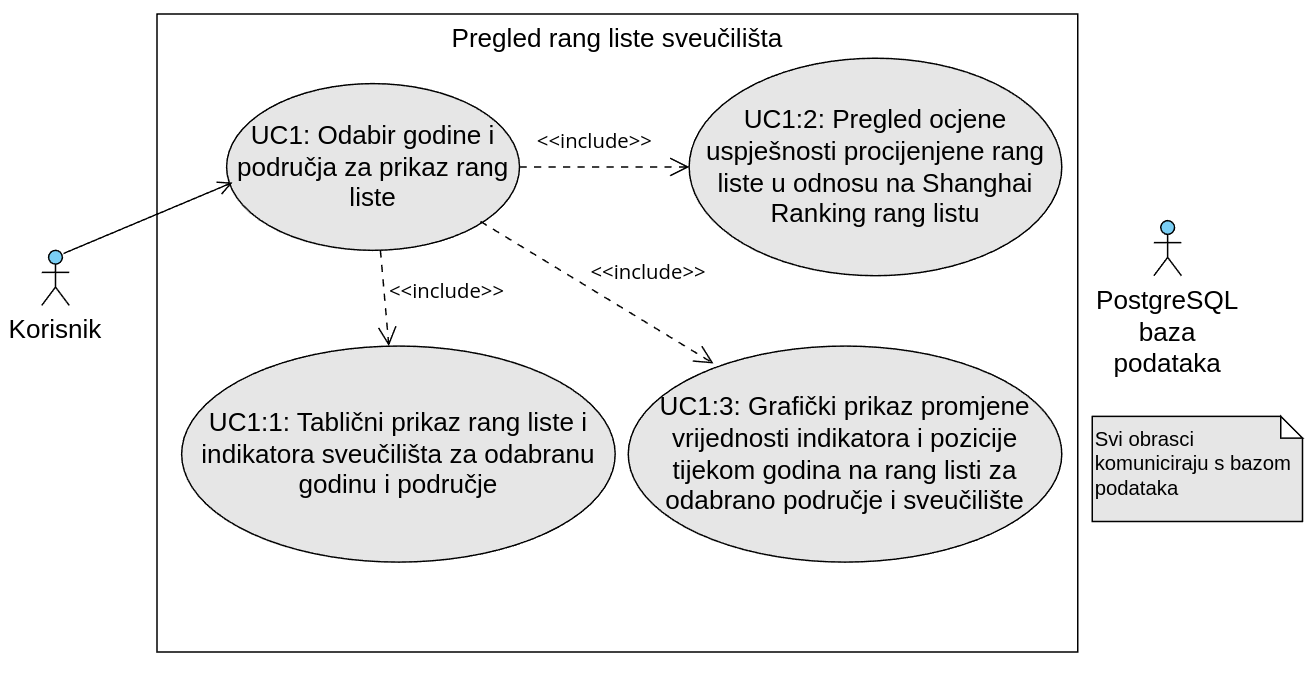
\includegraphics[scale=0.4]{slika1.png}
    \caption{Dijagram obrasca uporabe, korisnička funkcionalnost}
    \label{fig:korisnik}
    \end{figure}
\newpage
\section{Nefunkcionalni zahtjevi}
Nefunkcionalni zahtjevi opisuju koja svojstva sustav mora imati, a ne funkcionalnost koju pruža korisniku. Ova web aplikacija mora:

a) biti robusna, otporna na pogreške i stabilna

b) omogućiti brzo i fluidno korisničko sučelje

c) dati što bolju procjenu rankinga sveučilišta u odnosu na Shanghai Ranking sustav

\chapter{Korištene tehnologije}
\section{Arhitektura sustava}
Arhitektura ovog programskog sustava sastoji se kao i mnoge web aplikacije od 3 dijela:

1. web korisničko sučelje

2. \emph{backend} poslužitelj

3. baza podataka

\subsection{Web korisničko sučelje}
Web korisničko sučelje ove aplikacije napravljeno je u JavaScript biblioteci React. 
\\
\\ \textbf{React} je biblioteka otvorenog koda, razvijena od strane Facebooka,
prva verzija objavljena je 2013. godine te je danas vrlo raširena i često se koristi za izradu interaktivnih i dinamičkih web korisničkih sučelja. 
React omogućava jednostavniju izradu web aplikacija uz manje programiranja i manju složenost u odnosu na izradu web aplikacije u čistom JavaScriptu.
Jedna od prednosti React biblioteke je ta što omogućava izradu jednostraničnih web aplikacija \engl{Single Page Application (SPA)} koja radi tako 
da dinamički surađuje s preglednikom te navigiranje aplikacijom ne uzrokuje odlazak na potpuno drugačiju web stranicu već se trenutna stranica 
mijenja i prepisuje s podatcima dohvaćenih s web poslužitelja. Ovu funkcionalnost omogućava dodatak react-router-dom koji nudi komponente kao što su Link.
Navigiranjem po web aplikaciji korištenjem komponente Link mijenja se URL u pregledniku, ali web stranica zapravo ostaje ista uz promijenjen sadržaj.
React koristi virtualni DOM \engl{Document Object Model} koji prati stanja 
komponenti web stranice te kada dođe do promjene stanja, u stvarnom preglednikovom DOM-u mijenja samo one elemente koji su se promjenili. Ova 
funkcionalnost uvelike poboljšava performanse web aplikacije.
Jedna stranica u Reactu sastoji se od više manjih komponenti koje se mogu dijeliti između više stranica i proizvoljno gnijezditi. Ovakvom organizacijom
postiže se dobra organizacija koda uz mogućnosti višestrukog korištenja komponenti.
Kombiniranjem navedenih funkcionalnosti React biblioteke dobiva se fluidno korisničko sučelje bez puno ponovnih učitavanja stranica \engl{reload}.
\\
\\ \textbf{Axios}
\\ Axios je biblioteka koja omogućava jednostavno stvaranje HTTP zahtjeva kao što su GET i POST na \emph{backend} poslužitelj i rukovanje odgovorima koje taj poslužitelj vraća.
\\
\\ \textbf{Material UI}
\\ Pisanje vlastitih komponenti u Reactu od početka je korisno ako je potrebna potpuna kontrola nad komponentama te velika prilagodljivost, ali
često se koriste komponente s nekom generičkom funkcionalnosti te pisanje takvih komponenti svaki put od nule nije potrebno. 
Material UI je biblioteka za React koja nudi veliki broj gotovih komponenti koje se mogu prilagođavati i uređivati prema vlastitim potrebama .
\\
\\ \textbf{Tailwind CSS}
\\ Tailwind CSS je radni okvir \engl{framework} za CSS \engl{Cascading Style Sheets} koji ima niz gotovih CSS razreda koji omogućavaju lagano postizanje 
željenog izgleda komponenti.
\\
\\ \textbf{React-chartjs-2}
\\ React-chartjs-2 je jedna od najpopularnijih React biblioteka koja nudi funkcionalnost jednostavne izrade grafova. Koristi se za izradu grafova na 
kojima pratimo promjene ranking podataka tijekom vremena.
\\ \subsection{\emph{Backend} poslužitelj}
\textbf{Node.js} 
\\ Node.js je JavaScript pokretačko okruženje \engl{runtime environment} namijenjeno izvođenju na poslužiteljskoj strani. Pokreće se na V8 JavaScript \emph{engineu}
te omogućuje izvršavanje JavaScript koda izvan preglednika. Koristi asinkronu arhitekturu zasnovanu na događajima \engl{asynchronous event-driven architecture}
te nudi mogućnost izrade skalabilnih web aplikacija.\\\newpage \textbf{Express.js}
\\ Express.js je \emph{framework} Node.js-a te omogućava izradu RESTful API-ja \engl{Application Programming Interface}. Express.js nudi
lagano upravljanje HTTP zahtjevima i izradu krajnjih točaka \engl{endpoint} s kojima će React web aplikacija komunicirati.
\\ \\ \textbf{Puppeteer}
\\ Puppeteer je Node.js biblioteka koja nudi bogati API pomoću kojeg se preglednici Chrome i Chromium mogu kontrolirati koristeći DevTools protokol.
DevTools protokol omogućuje alatima upravljanje preglednicima kao što su Chrome i Chromium na temelju uputa koje smo dali tim alatima.
Puppeteer koristimo za izradu \emph{web scrappera} (alat koji posjećuje web stranice i 
na njima obavlja neke radnje bez potrebe za intervencijom čovjeka) za baze InCites i WoS. Iako navedene baze nude API pomoću kojeg bi mogli 
dohvatiti sve podatke potrebne za ranking, on se plaća. Puppeteer alatu moramo zadati niz koraka koje treba obaviti na nekoj stranici (upisati tekst u neko polje, pritisnuti na gumb, otići na drugu stranicu)
kako bi postigli željeni rezultat.
\\ \\ \textbf{Node-postgres} 
\\ Kako bi \emph{backend} poslužitelj mogao komunicirati s bazom podataka koristi se Node-postgres. To je skup Node.js modula koji nude 
sučelje prema bazi podataka. Pomoću ovog proširenja s \emph{backend} poslužitelja se mogu raditi sve uobičajene radnje s bazom podataka (stvaranje novih tablica, 
unos podataka u tablice, dohvaćanje podataka iz tablica, brisanje podataka iz tablica i razne druge radnje).
\\ \\ \textbf{Node Cron}
\\ Node Cron je Node.js modul koji omogućava obavljanje nekih radnji na \emph{backend} poslužitelju u željeno vrijeme. Node Cron modul se u ovoj 
web aplikaciji koristi kako bi se svaka dva tjedna pokrenuo alat Puppeteer koji će prikupiti najnovije podatke za ranking sveučilišta.
\\ \subsection{Baza podataka}Ova web aplikacija koristi relacijsku bazu podataka otvorenog koda PostgreSQL. \\PostgreSQL baza podataka ima ACID 
\engl{Atomicity, Consistency, Isolation, Durability} svojstva koja su bitna kako bi se osigurala robusnost i stabilnost web aplikacije.
\\ \section{Docker}
Kako bi se ova web aplikaciju mogla lako postaviti \engl{deploy} na neki poslužitelj te tako omogućiti svim korisnicima pristup aplikaciji,
koristi se platforma Docker. Docker je platforma otvorenog koda koja se koristi za razvoj, isporuku i pokretanje aplikacija.
Docker pakira dijelove web aplikacije u odvojene dijelove koji se zovu kontejneri \engl{containers}.
Kontejneri su zapravo Docker slike \engl{images} u izvođenju. Docker slika je lagana \engl{lightweight} komponenta koja sadrži sve što je aplikaciji 
potrebno za izvođenje (izvorni kod, pokretačko okruženje \engl{runtime}, razne alate i biblioteke). Način stvaranja docker slike se definira 
datotekom \\Dockerfile. Jednom kad je stvorena Docker slika, može se pokrenuti. Time se dobije kontejner koji se izvršava na Docker Engineu. 
Velika prednost Dockera je ta što je podržan na puno operacijskih sustava (Windows, Linux, MacOS i ostali) te uz pomoć samo jedne naredbe i datoteke Dockerfile
dobije se pokrenuta i funkcionalna aplikacija. Aplikacije koje se pokreću kao kontejneri rade na jednak način na svim operacijskim sustavima zbog ugrađene virtualizacije.
Docker virtualizira operacijski sustav, a ne sklopovlje. Ovo je velika prednost u odnosu na virtualizaciju koju rade virtualni strojevi. 
Virtualni strojevi emuliraju sklopovlje i upravljanjem pomoću hipervizora omogućuju da se na istom sklopovlju izvršava više operacijskih sustava. 
Docker kontejneri dijele isti operacijski sustav te svaki predstavlja poseban proces. Docker kontejneri zauzimaju manje 
resursa, lakši su i brži. 

\begin{figure}[htb]
    
    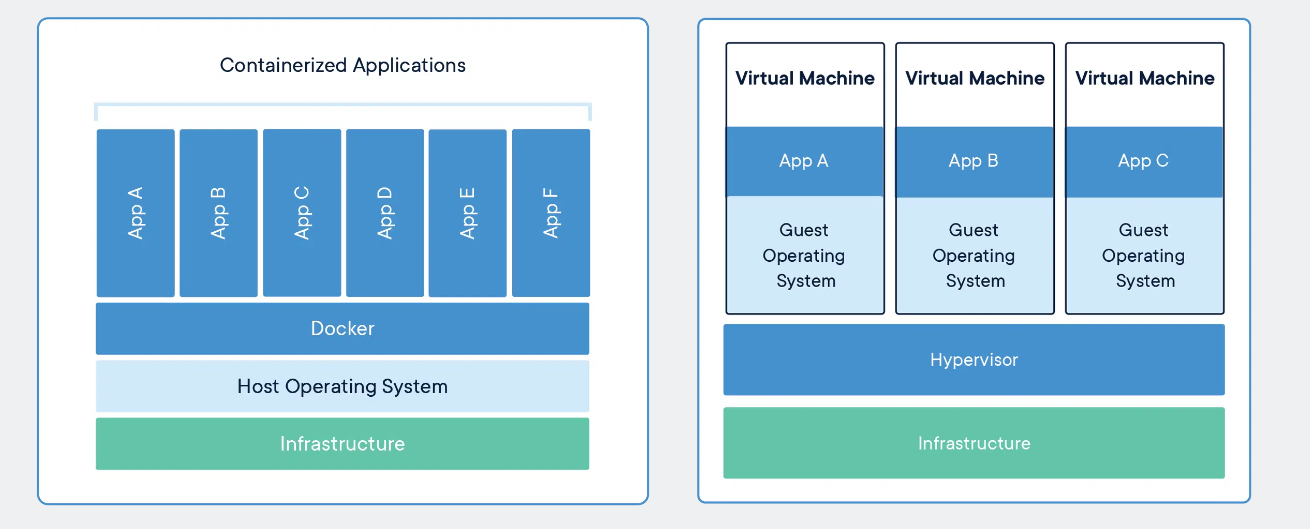
\includegraphics[scale=0.35]{slika2.png}
    \caption{Usporedba virtualnih strojeva i Docker načina virtualizacije}
    \label{fig:docker}
    \end{figure}

U slučaju ove aplikacije postoje 3 Docker slike koje će postati Docker kontejneri prilikom izvođenja. Jedna slika je za bazu podataka,
druga za \emph{backend} poslužitelj, a treća za web korisničko sučelje. Jednom kada je napisan Dockerfile za sve navedene dijelove aplikacije, dijelovi se povezuju  
datotekom docker-compose. U toj datoteci stoje upute od kojih se sve kontejnera aplikacija sastoji, kako kontejneri međusobno surađuju te kako se pokreću. Zahvaljujući 
ovoj datoteci, umjesto da se svaki kontejner posebno inicijalizira i pokrene, s jednom naredbom se pokrene cijela aplikacija.
\\
\begin{figure}[htb]
    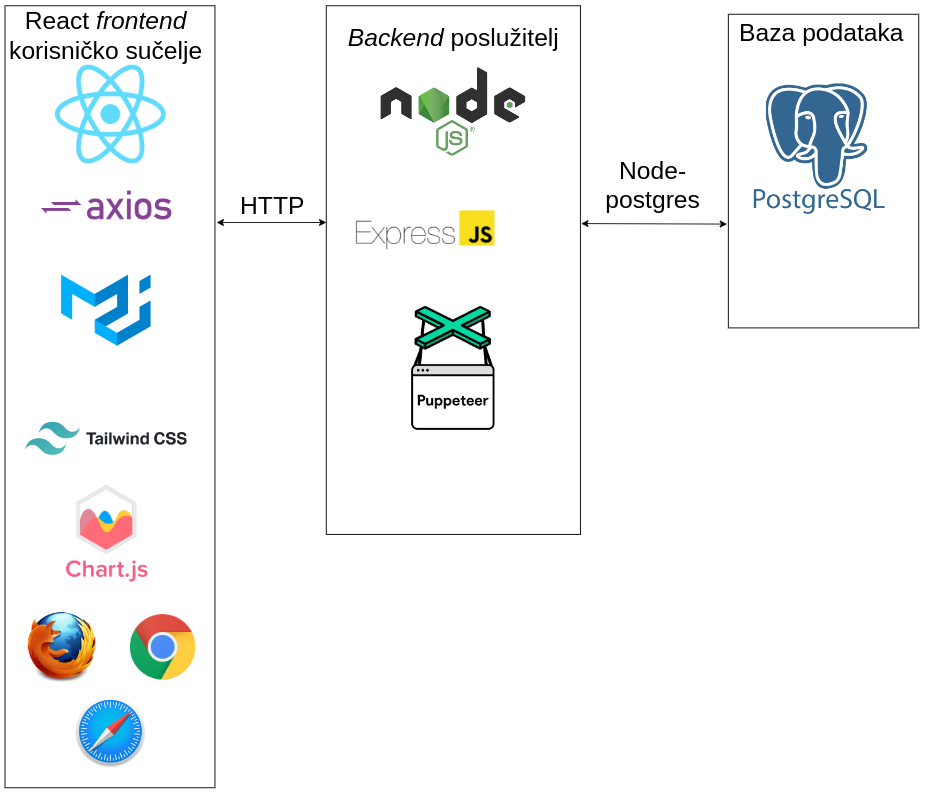
\includegraphics[scale=0.3]{tehnologije.png}
    \caption{Prikaz raspodjele korištenih tehnologija po arhitekturnim slojevima}
    \label{fig:arhitektura}
    \end{figure}
\chapter{Pregled funkcionalnosti}
\section{Početna stranica}

\begin{figure}[htb]
    \hspace*{-2cm}  
    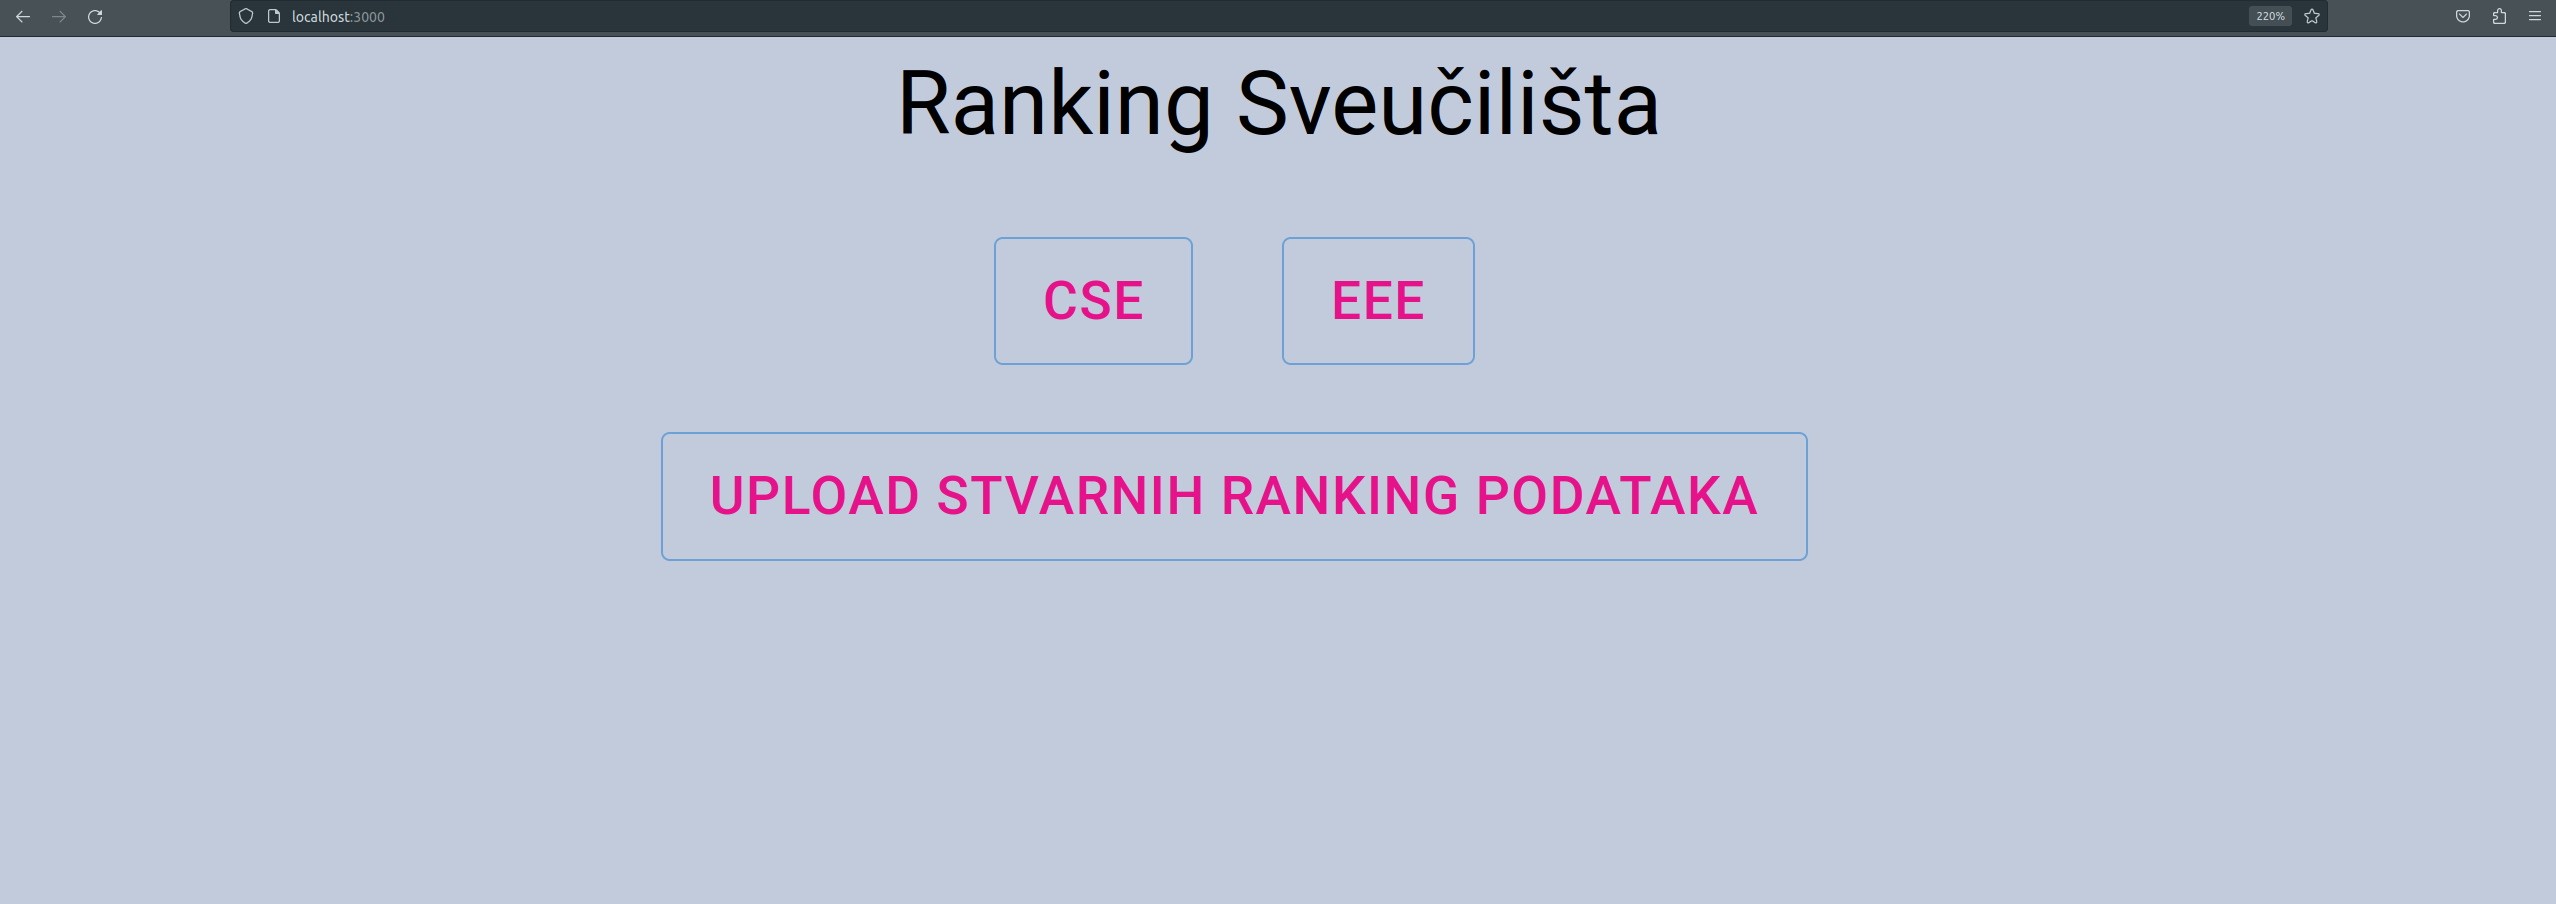
\includegraphics[scale=0.2]{homePage.png} 
    \caption{Prikaz početne stranice}
    \label{fig:homepage}
    \end{figure}
Početna stranica nalazi se na putanji "/". Na početnoj stranici korisnik može birati između tri opcije. Pritiskom na neki od gornja dva gumba \emph{CSE} ili \emph{EEE}
korisnika će se preusmjeriti na stranicu za pregled procjene Shanghai Rankinga i svih vrijednosti indikatora za područje CSE, odnosno EEE.        
Pritiskom na donji gumb \emph{UPLOAD STVARNIH RANKING PODATAKA} korisnik će biti preusmjeren na stranicu na kojoj može objaviti .xlsx datoteku koja ima 
identične vrijednosti indikatora i pozicija za pojedina sveučilišta kao i Shanghai Ranking stranica. Na osnovu te datoteke popunit će se baza podataka, a 
objavljeni podatci služit će za usporedbu procjene rankinga i Shanghai Rankinga.  
\newpage\section{Tablični prikaz rankinga sveučilišta}
\begin{figure}[htb]
    \hspace*{-2cm}  
    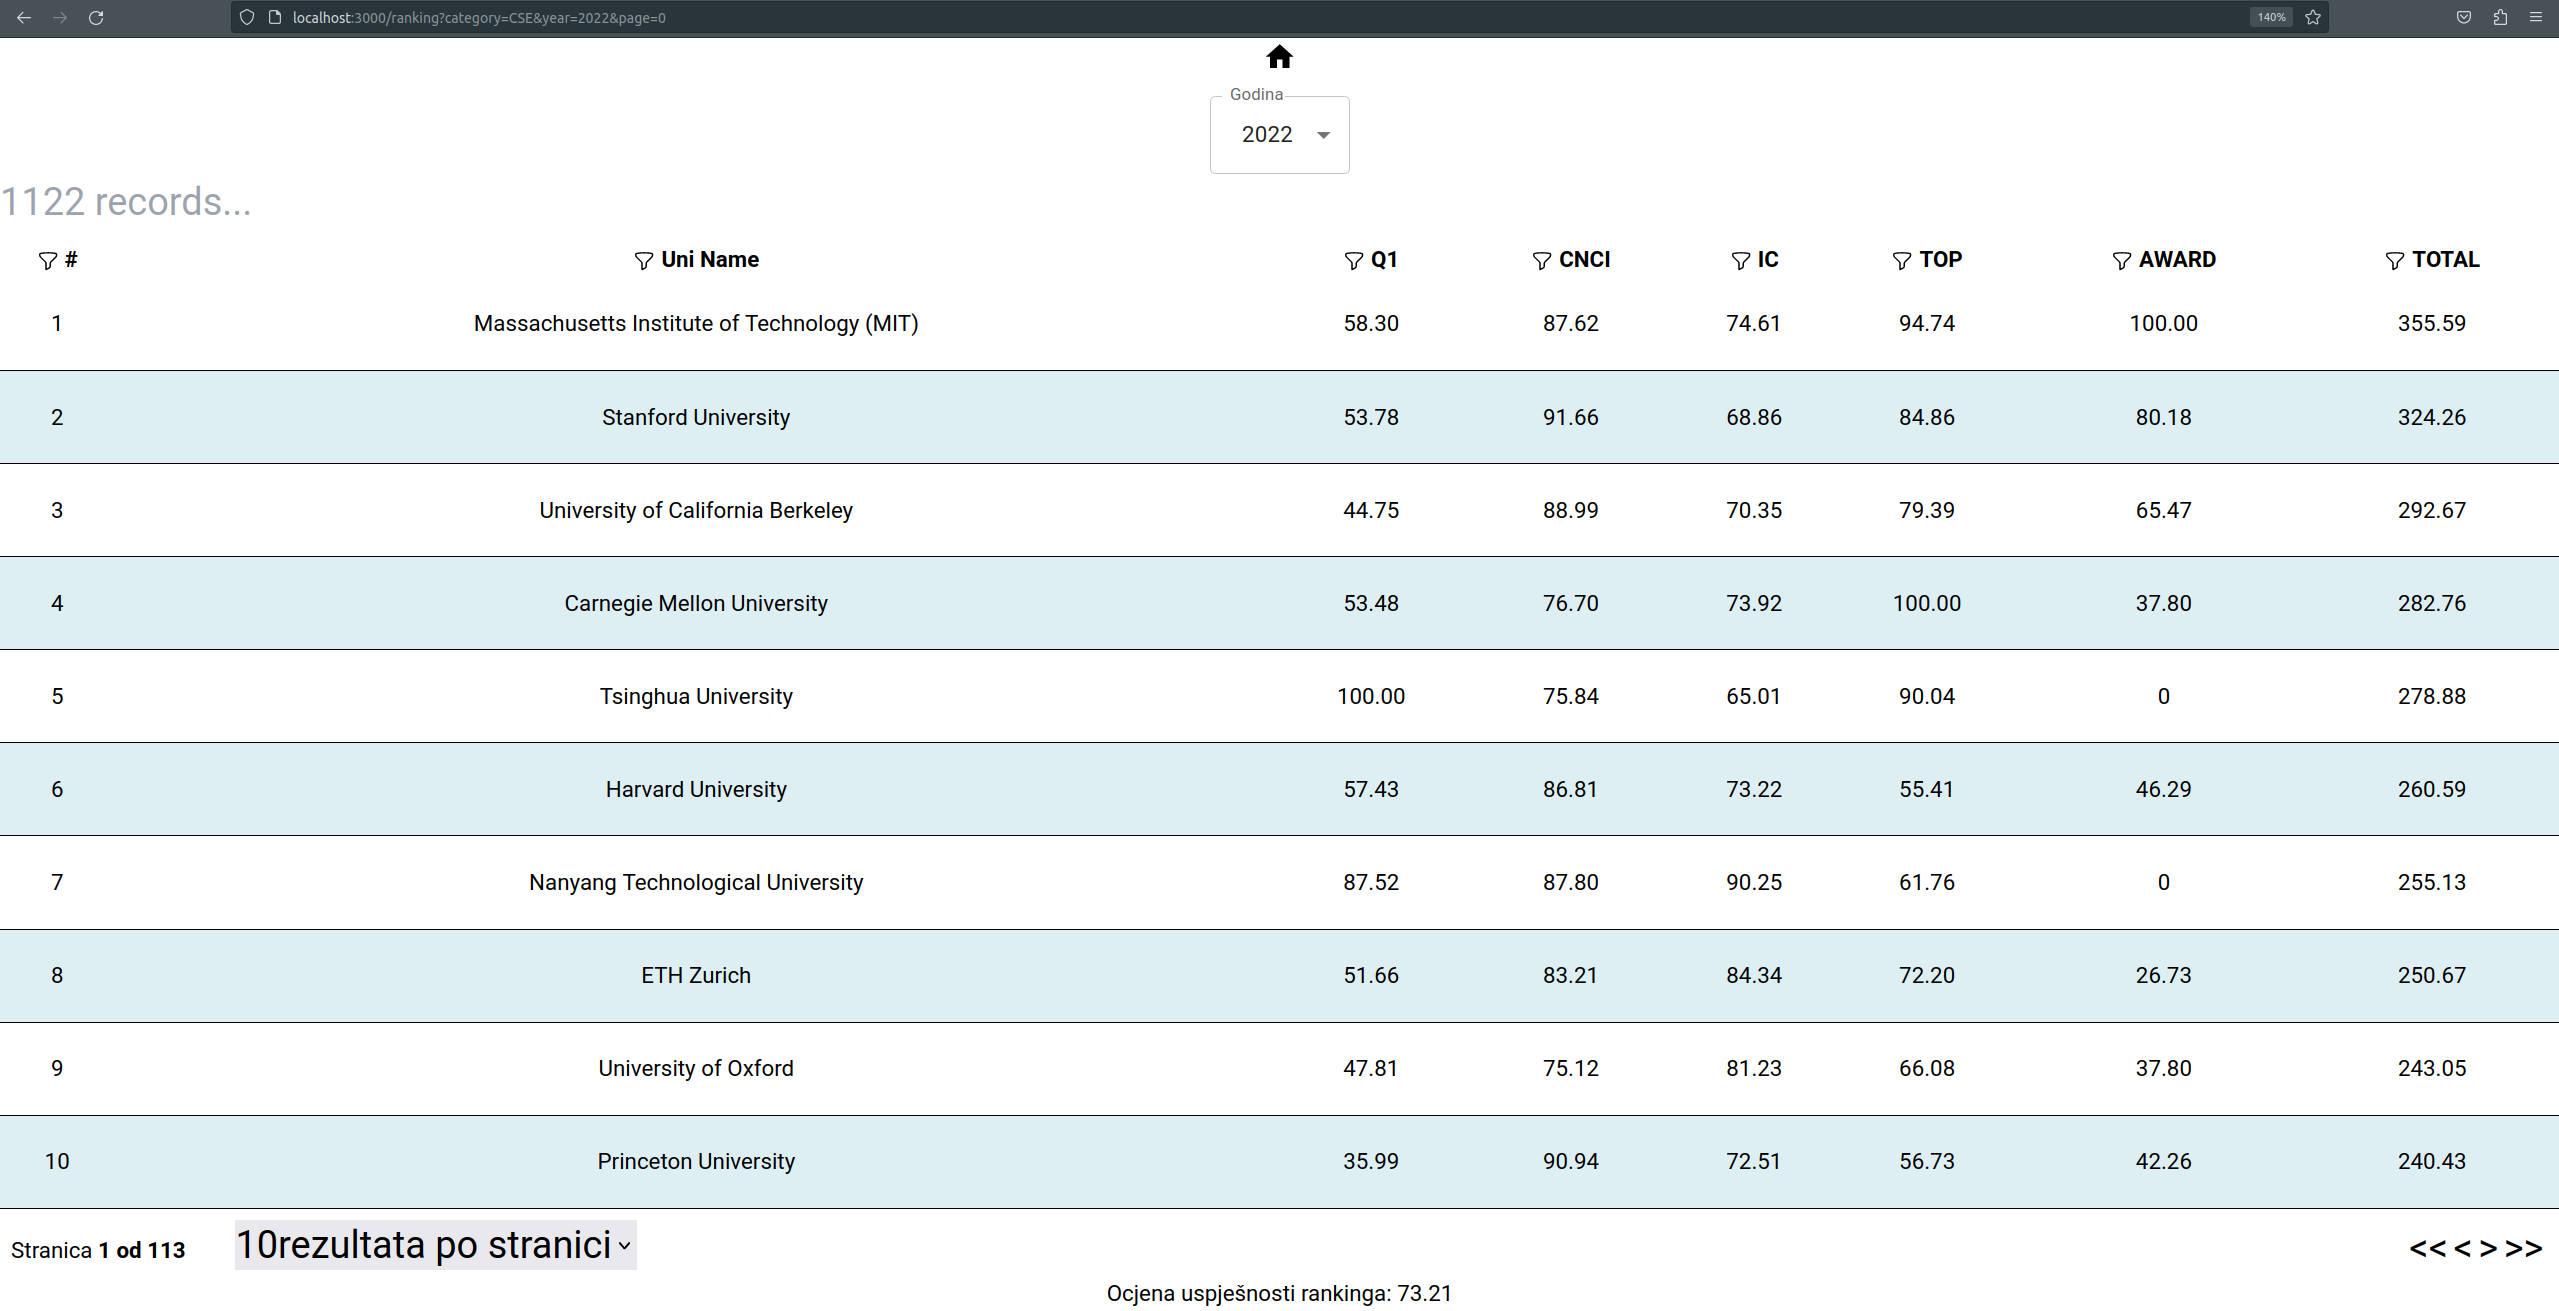
\includegraphics[scale=0.2]{tablica.png} 
    \caption{Tablični prikaz rankinga sveučilišta}
    \label{fig:tablica}
    \end{figure}

Pritiskom na neki od gumba \emph{CSE} ili \emph{EEE} korisniku se prikaže stranica na slici \ref{fig:tablica}. Putanja koja vodi do ove stranice 
je "/ranking?category=CSE\&year=2022\&page=0".
URL parametar \emph{category} specifira za koje područje se prikazuje procjena rankinga, parametar \emph{year} specifira 
za koju godinu se gleda procjena rankinga, a parametar \emph{page} je pomoćni parametar za ostvarenje paginacije.  
U ovom konkretnom primjeru iz URL-a se vidi da korisnik trenutno gleda prvu stranicu (indeksiranje stranica kreće od 0) procjene rankinga sveučilišta u području CSE za 2022.godinu.
\\Stranica na vrhu ima ikonu u obliku kućice s kojom se korisnik vraća na početnu stranicu. \\Odmah ispod ikone kućice nalazi se komponenta
za odabir godine za koju korisnik želi pogledati procjenu rankinga sveučilišta. Pritiskom na tu komponentu prikazuje se padajući izbornik 
s popisom godina od 2017. godine do trenutne godine. 
\begin{figure}[htb]
    \centering
       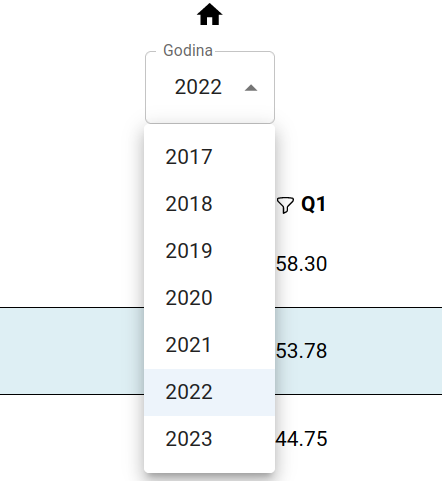
\includegraphics[scale=0.24]{select.png} 
       \caption{Komponenta za odabir godine za koju se prikazuju podatci procjene rankinga}
       \label{fig:select}
       \end{figure}
Početna godina je 2017. jer od te godine su dostupne rang liste na stranici 
Shanghai Ranking. Kada korisnik odabere jednu od ponuđenih godina u URL-u se mijenja parametar \emph{year}, šalje se HTTP GET zahtjev na \emph{backend}
poslužitelj te se ažurira tablica procjene rankinga s podatcima za odabranu godinu koje \emph{backend} poslužitelj pošalje u HTTP odgovoru \engl{response}.
\newpage Ispod komponente za odabir godine, a prije tablice rankinga
nalazi se polje za pretragu sveučilišta po njihovom imenu. Prije nego što korisnik krene upisivati slova u to polje, u njemu kao zamjenski tekst \engl{placeholder}
piše koliko sveučilišta se određene godine u nekom području našlo na procijenjenoj rang listi. Na slici \ref{fig:tablica} se vidi da je za 2022. godinu u području CSE 
na procijenjenoj rang listi 1122 sveučilišta.
Upisom imena sveučilišta u tablici za procjenu rankinga pojavit će se podatci samo za ona sveučilišta
koja u imenu sadrže podniz koji je korisnik upisao u polje za pretragu. Upisom podniza na \emph{backend} poslužitelj HTTP GET zahtjevom šalje se taj podniz te se 
pretražuje baza podataka procijene rankinga za određenu godinu u nekom području po imenu sveučilišta. Dolaskom HTTP odgovora ažuriraju se podatci u tablici.\\
\begin{figure}[htb]
    \hspace*{-2cm}  
       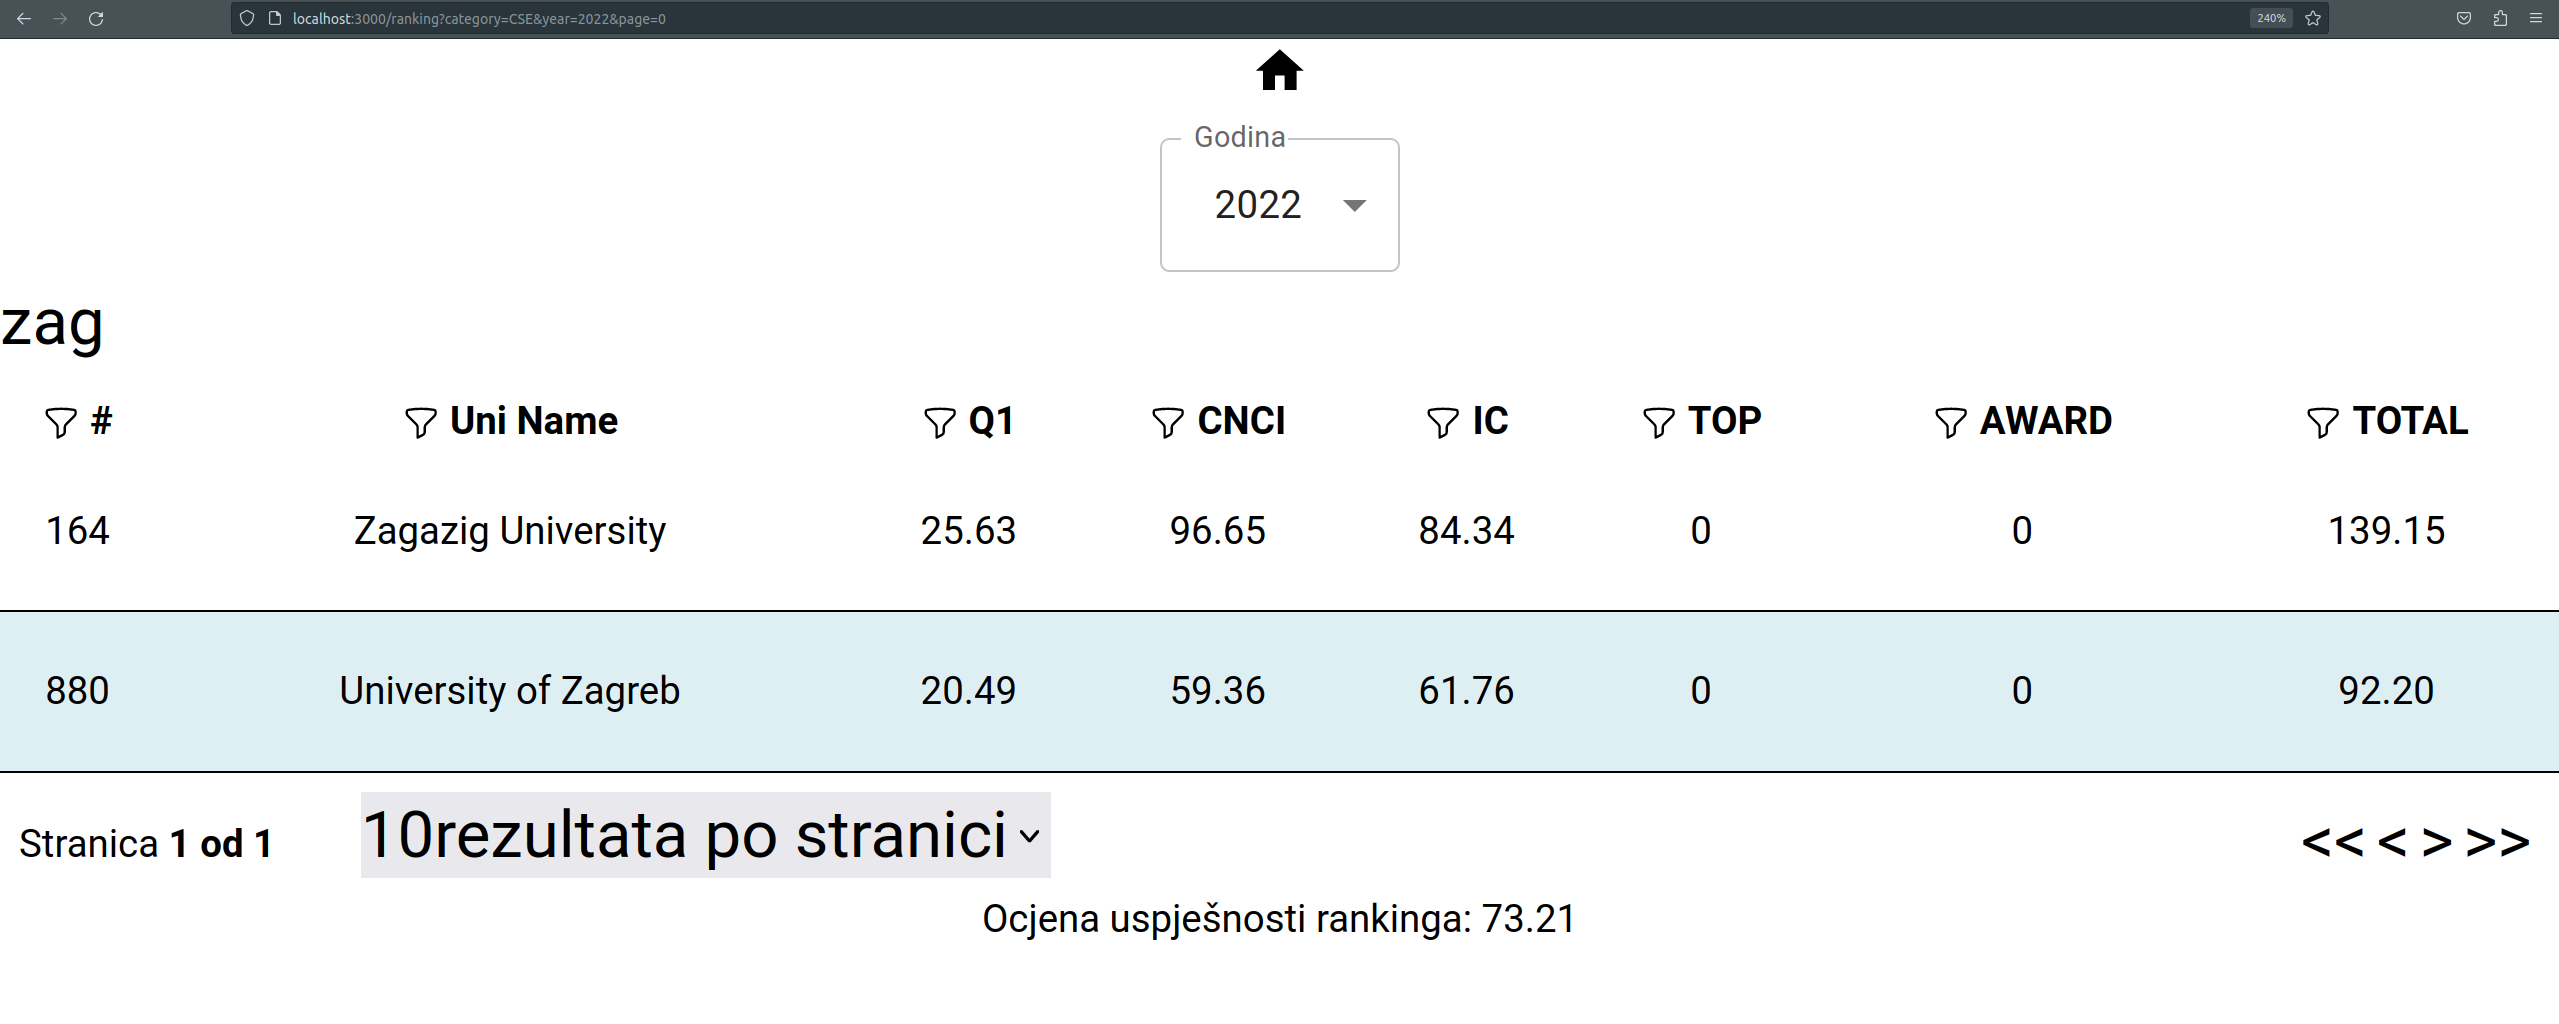
\includegraphics[scale=0.21]{search.png} 
       \caption{Primjer pretrage sveučilišta po imenu}
       \label{fig:search}
       \end{figure}
\\Na slici \ref{fig:search} se vidi primjer pretrage sveučilišta po imenu. Korisnik je upisao niz slova "zag" te se u tablici vide podatci za dva sveučilišta
koja u svom imenu sadrže navedeni podniz. 
\\Tablica procjene rankinga sastoji se od 8 stupaca. Zaglavlje tablice sadrži nazive vrijednosti koje se nalaze u pojedinim stupcima.
Prvi stupac pokazuje poziciju sveučilišta na rang listi za određenu godinu te u nekom području, drugi 
pokazuje ime sveučilišta, sljedećih pet stupaca sadrže vrijednosti koje se vežu uz indikatore Q1, CNCI, IC, Top i Award, a zadnji stupac sadrži ukupan rezultat sveučilišta 
u određenoj godini za neko područje prema kojem su sveučilišta sortirana i zove se Total. U zaglavlju tablice prije samog naziva vrijednosti stupca nalazi se ikona koja simbolizira
sortiranje tablice rankinga. Ova funkcionalnost omogućena je za sve stupce osim prva dva. Ako korisnik pritisne na tu ikonu ili naziv stupca cijela tablica 
procjene rankinga sortirat će se prema vrijednosti tog stupca silazno odnosno uzlazno. 
\begin{figure}[htb]
    \hspace*{-2cm}  
       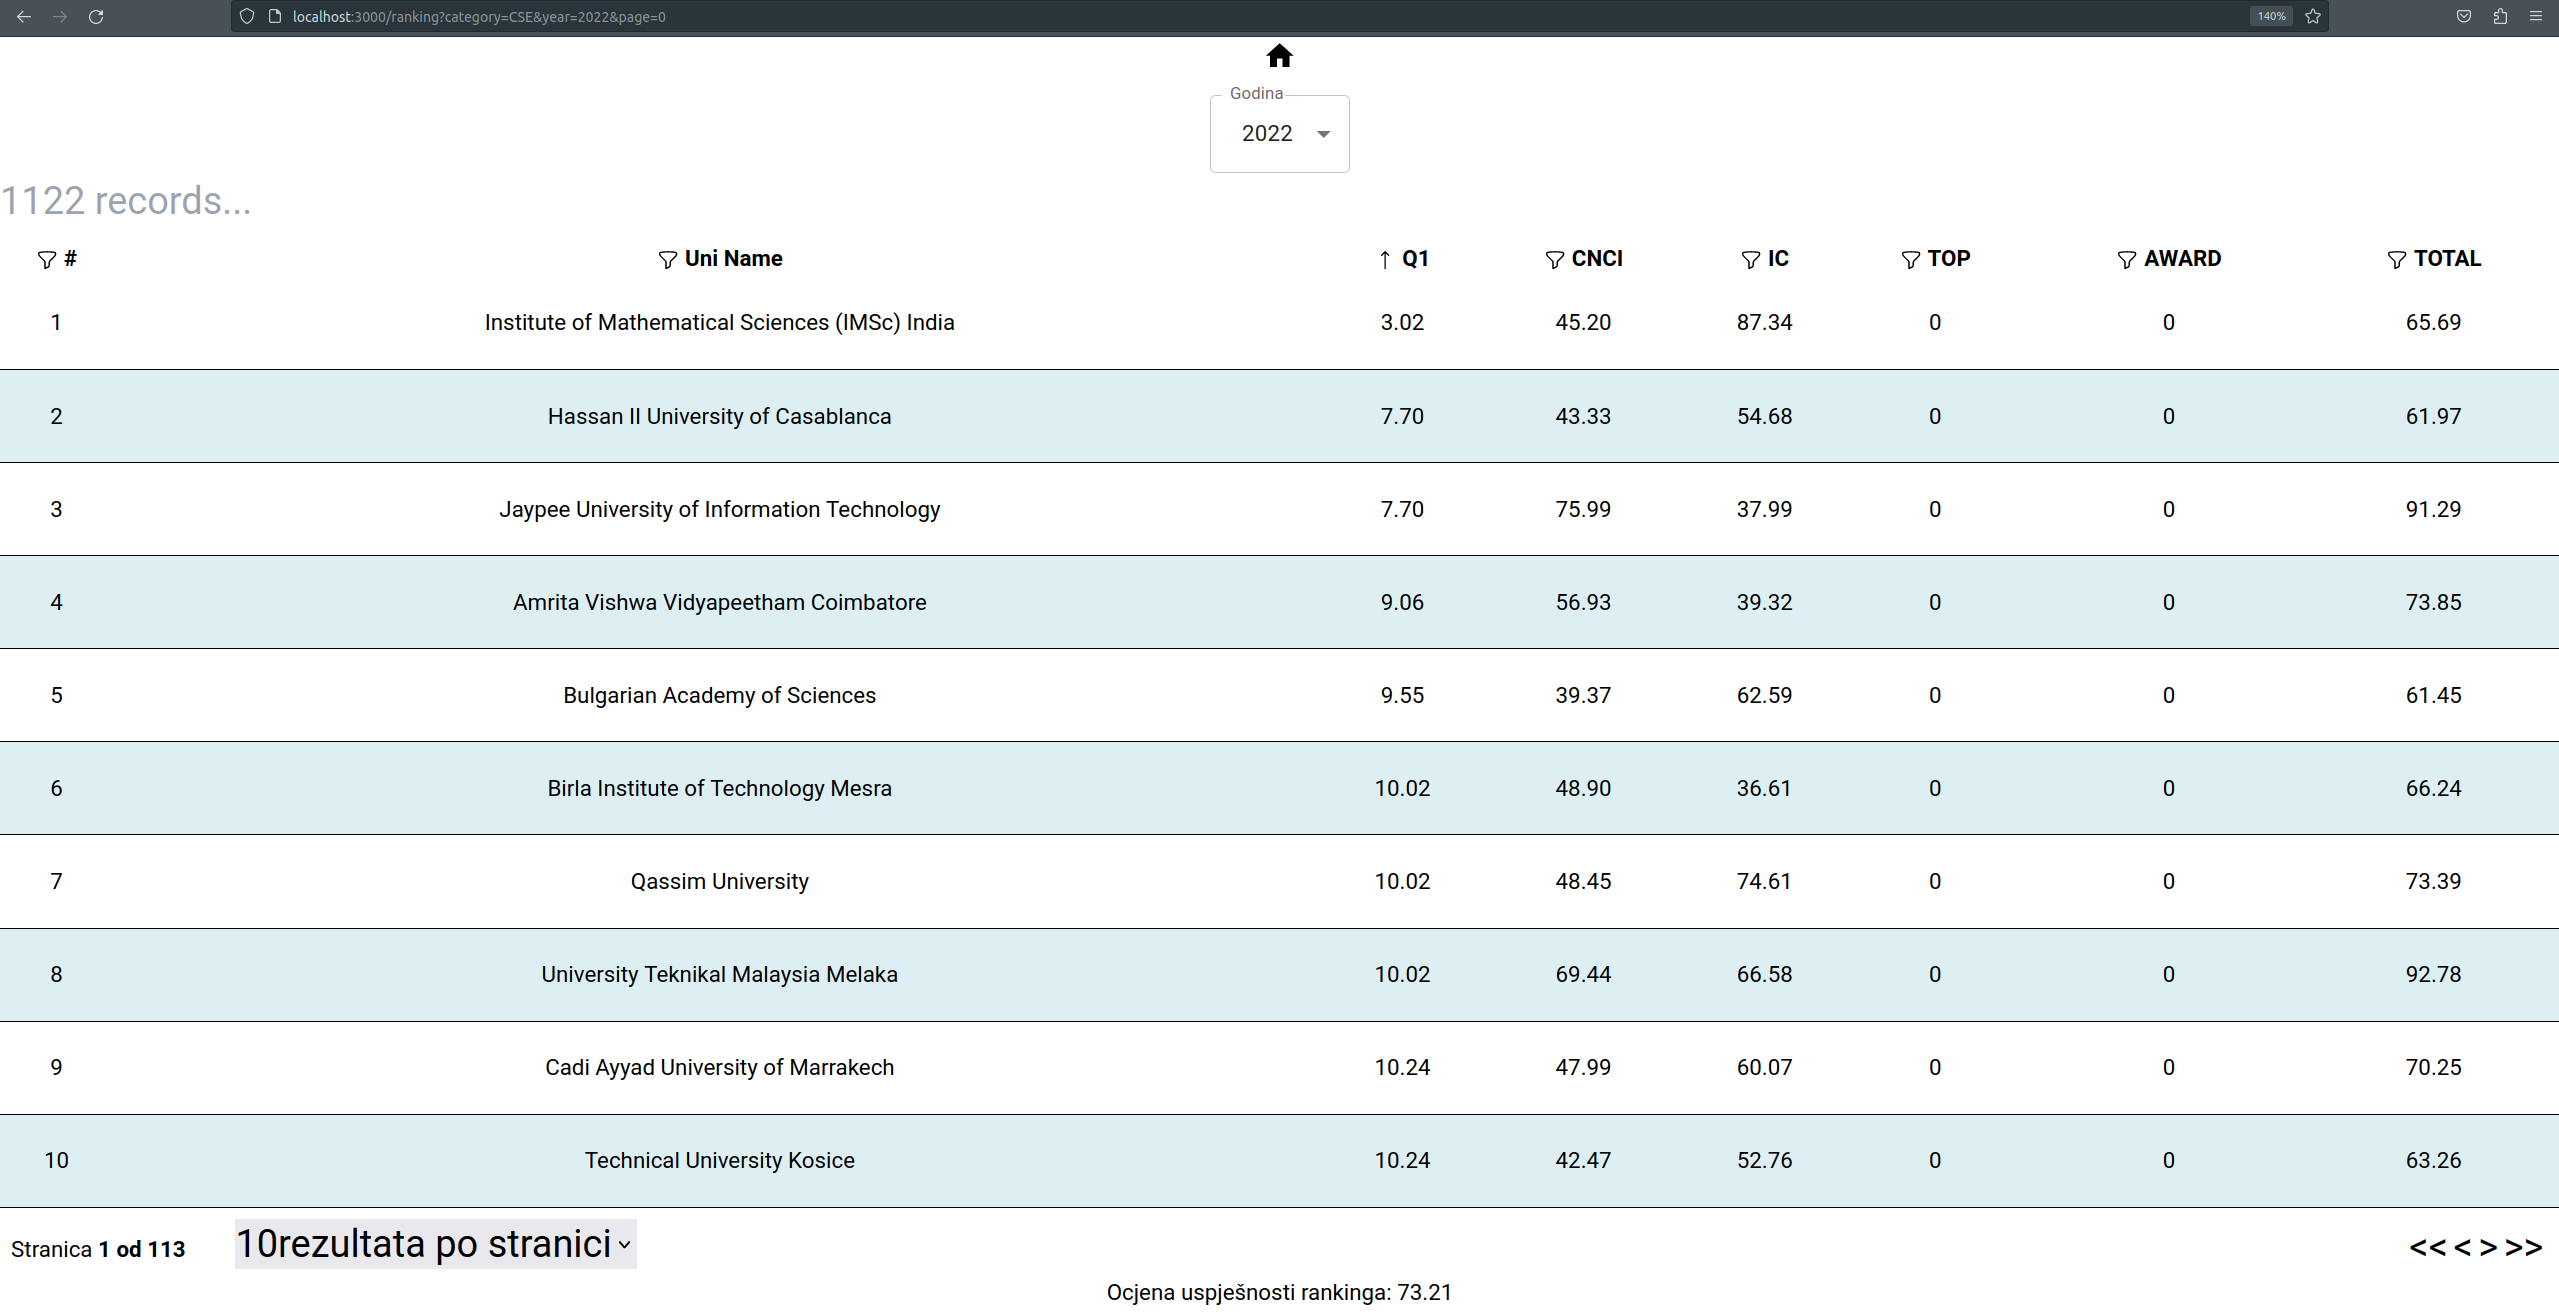
\includegraphics[scale=0.21]{sort1.png} 
       \caption{Primjer uzlaznog sortiranja tablice procjene rankinga prema vrijednosti indikatora Q1}
       \label{fig:sort1}
       \end{figure}
\\Slika \ref{fig:sort1} prikazuje stanje tablice nakon što je korisnik pritisnuo u zaglavlju tablice treći stupac koji ima naziv Q1. Sada se ikona koja simbolizira
sortiranje zamjenila s ikonom strelice koja pokazuje prema gore. Strelica prema gore simbolizira da se cijela tablica procjene rankinga
sortira uzlazno prema vrijednosti indikatora uz koji se nalazi strelica, u ovom slučaju to je indikator Q1. Sada su se podatci u tablici 
ažurirali te su sveučilišta sortirana uzlazno po vrijednosti indikatora Q1 što se i vidi u samoj tablici na slici \ref{fig:sort1} jer vrijednost indikatora Q1 za prvo 
sveučilište je 3.02, a za svako sljedeće sveučilište ta vrijednost je veća u odnosu na prethodno sveučilište. Sortiranje se može raditi i silazno. Tada se ikona promjeni
u strelicu koja je okrenuta prema dolje. Promjene vrste sortiranja između silaznog, uzlaznog ili zadanog \engl{default} se radi uzastopnim pritiskanjem 
jednog od zadnjih 6 stupaca u zaglavlju tablice.
\begin{figure}[htb]
    \hspace*{-2cm}  
       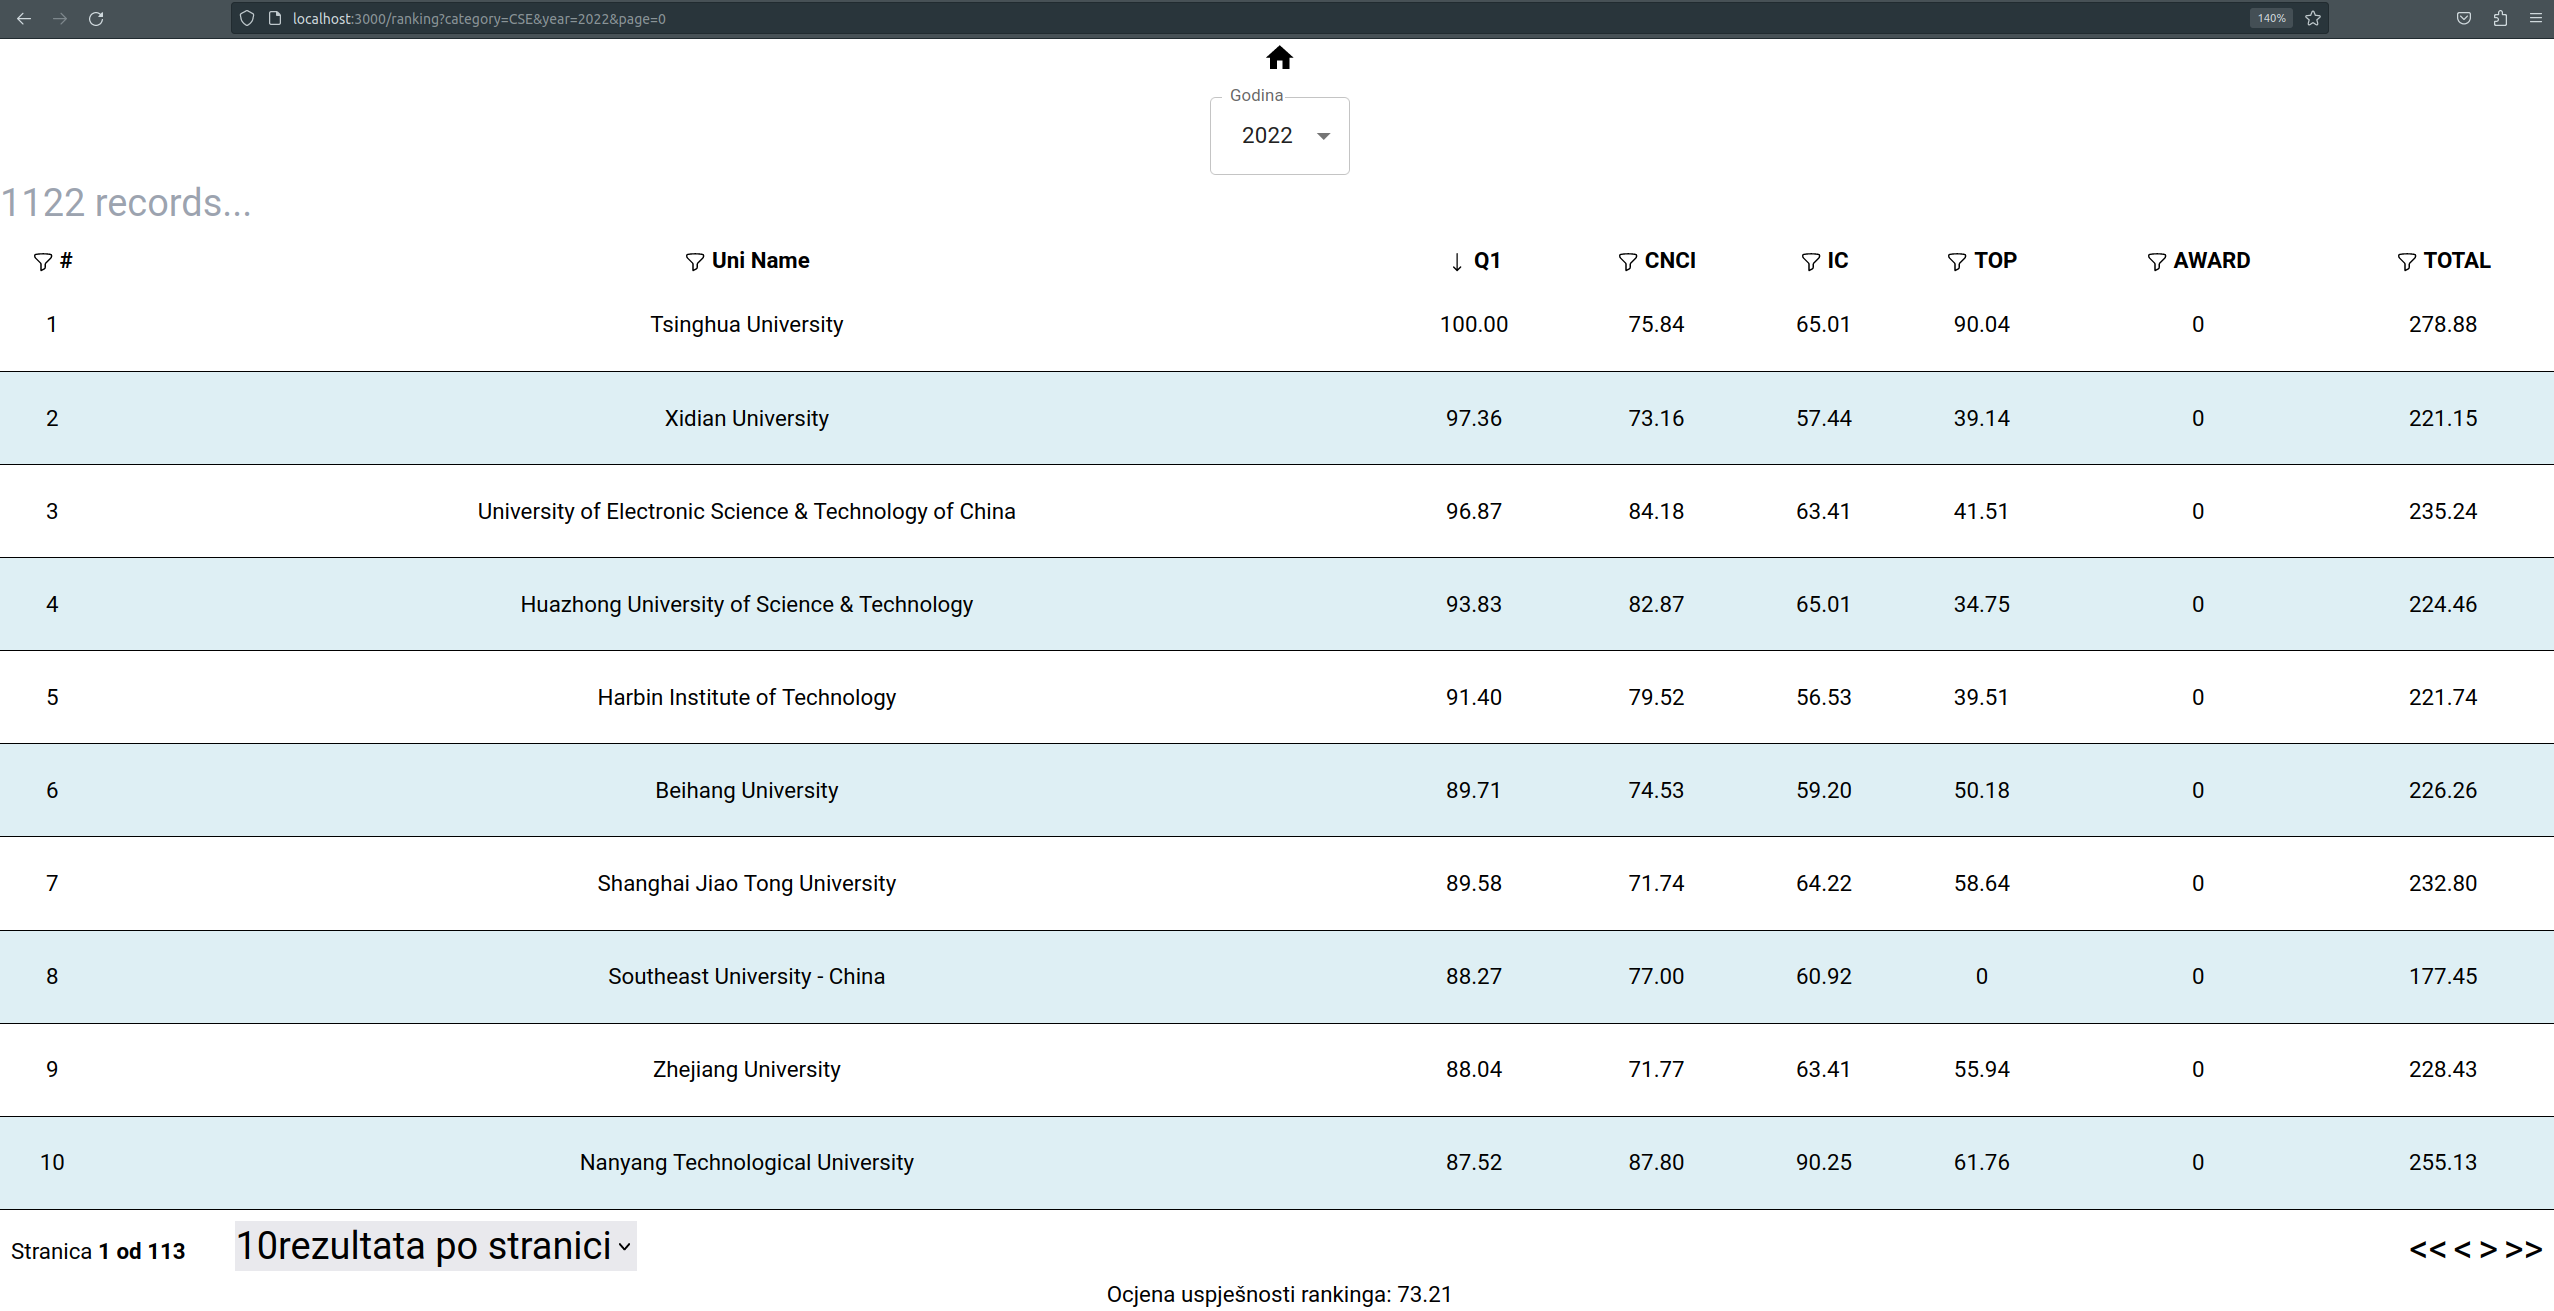
\includegraphics[scale=0.21]{sort2.png} 
       \caption{Primjer silaznog sortiranja tablice procjene rankinga prema vrijednosti indikatora Q1}
       \label{fig:sort2}
       \end{figure}
\\\engl{Default} sortiranje je silazno prema vrijednosti stupca Total jer se tako dobije rang lista sveučilišta od najboljih prema najgorim uzimajući u obzir sve 
vrijednosti koje se vežu uz pojedine indikatore.
Istodobno sortiranje sveučilišta prema više vrijednosti stupaca nije moguće. Tako na primjer ako korisnik prvo odabere uzlazno sortiranje prema vrijednosti stupca 
Q1 te zatim odabere sortiranje za stupac IC, sortiranje prema vrijednosti stupca Q1 će se poništit te će se primjeniti željeno sortiranje prema vrijednosti stupca IC.
Sortiranje sveučilišta se također odvija na 
\emph{backend} poslužitelju, a parametri se prenose u sklopu HTTP GET zahtjeva. Dolaskom HTTP odgovora ažuriraju se podatci u tablici.
\\Zbog potencijalno velikog broja sveučilišta na rang listama, korisniku se ne prikažu sva sveučilišta u obliku jedne velike tablice nego 
je napravljena paginacija tako da se na jednoj stranici prikaže samo određeni broj zapisa iz rang liste sveučilišta. Informacija o tome na kojoj je trenutno stranici i 
koliko ukupno stranica rang liste ima korisniku je vidljiva ispod tablice uz lijevi rub. 
\begin{figure}[htb]
    \centering
       
\includegraphics[scale=0.3]{stranica.png} 
       \caption{Prikaz trenutne stranice i ukupnog broja stranica rang liste}
       \label{fig:paginacija}
       \end{figure}
\\Korisnik također može birati količinu redaka tablice po jednoj stranici. Pritiskom na komponentu ispod tablice otvara se 
izbornik gdje korisnik može birati između 10, 20, 30, 40 ili 50 redaka tablice po jednoj stranici. \emph{Default} vrijednost je 10. Ova vrijednost zajedno s 
trenutnim brojem stranice prenose se kao parametri prilikom HTTP GET zahtjeva kako bi \emph{backend} poslužitelj znao koliko zapisa i s kojim pomakom mora vratiti u 
HTTP odgovoru klijentu. Na ovaj način na klijentskoj strani imamo pohranjeno uvijek najviše 50 zapisa što pridonosi brzini korisničkog sučelja.
\begin{figure}[htb]
    \centering
       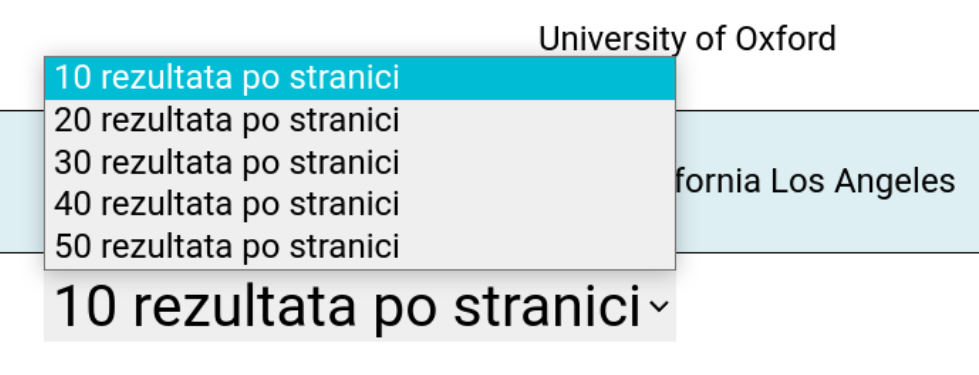
\includegraphics[scale=0.3]{brojstranica.png} 
       \caption{Odabir broja redaka tablice po jednoj stranici rang liste}
       \label{fig:brojstranica}
       \end{figure}
\\Ispod tablice rankinga uz desni rub nalazi se područje za navigiranje stranicama rang liste.       
\begin{figure}[htb]
    \centering
       
\includegraphics[scale=0.4]{navigiranje.png} 
       \caption{Područje za navigiranje stranicama rang liste}
       \label{fig:navigacija}
       \end{figure}
Postoje četiri mogućnosti navigacije kao što se i vidi na slici \ref{fig:navigacija}. Pritiskom na ikonu označenu brojem 1 korisniku će se prikazati prva stranica rang liste.
Pritiskom na ikonu označenu brojem 2 korisnik će se pomaknuti za jednu stranicu unazad, a pritiskom na ikonu označenu brojem 3 prikazat će se sljedeća stranica. 
Pritisci na ikone 2 i 3 funkcioniraju ukoliko uistinu postoji prethodna odnosno sljedeća stranica, u suprotnom se ništa ne događa.
Pritiskom na zadnju ikonu označenu rednim brojem 4 korisniku će se prikazati zadnja stranica rang liste. 
\\Ako je korisnik recimo navigirao na petu stranicu rang liste te u tom trenutku krenuo pretraživati sveučilišta, automatski ga se navigira na prvu stranicu rang liste.
\\Prilikom ažuriranja prikaza tablice rankinga ne dolazi do ponovnog učitavanja stranice što je jedna od opisanih koristi jednostraničnih web aplikacija.
Za vrijeme čekanja HTTP odgovora od \emph{backend} polsužitelja korisniku se prikaže odgovarajuća ikona te se pozadina posivi.
\begin{figure}[htb]
    \hspace*{-2cm}  
       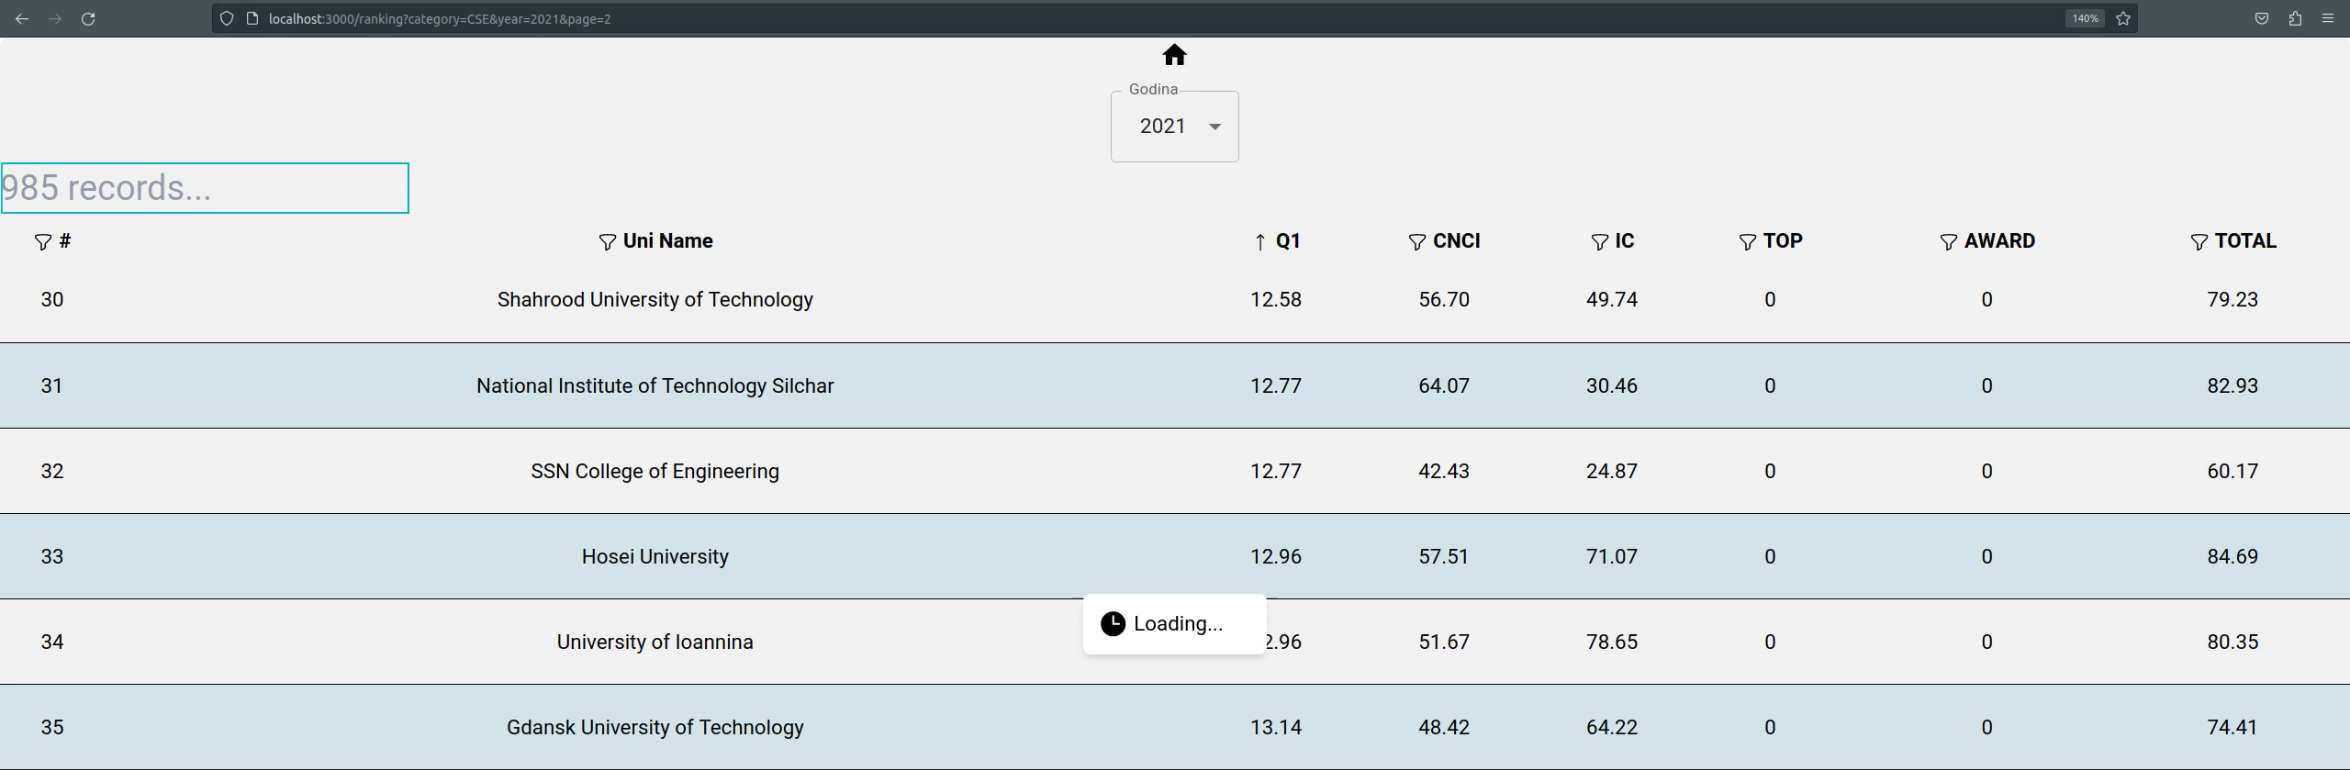
\includegraphics[scale=0.21]{loading.png} 
       \caption{Primjer čekanja HTTP odgovora \emph{backend} poslužitelja}
       \label{fig:sort2}
       \end{figure}
\\Na samom dnu stranice nalazi se ocjena uspješnosti procjene rankinga za neku godinu u određenom području u odnosu na stvarni 
ranking objavljen na stranici Shanghai Ranking. To je decimalni broj u rasponu od 0 do 100. Što je vrijednost tog broja veća znači da se procjena 
rankinga to bolje podudara sa stvarnim ranking podatcima sa Shanghai Ranking stranice. 
\begin{figure}[htb]
    \centering
       
\includegraphics[scale=0.4]{uspjeh.png} 
       \caption{Labela sa ocjenom uspješnosti procjene rankinga}
       \label{fig:uspjeh}
       \end{figure}
\\Na svako ime sveučilišta u tablici rankinga korisnik može pritisnuti mišem te će ga se preusmjeriti na stranicu s detaljnijim podatcima za to konkretno sveučilište.
\section{Stranica sveučilišta}
Temeljni funkcionalni zahtjevi su bili da korisnik može pratiti ranking sveučilišta i promjene vrijednosti indikatora tijekom godina, pogledati procjenu 
rankinga sveučilišta u tekućoj godini te usporediti procjenu rankinga sa stvarnim ranking podatcima na \\stranici Shanghai Ranking. Ova stranica 
nudi te funkcionalnosti korisniku u obliku grafičkog prikaza. 
\\
\begin{figure}[htb]
    \hspace*{-2cm}  
       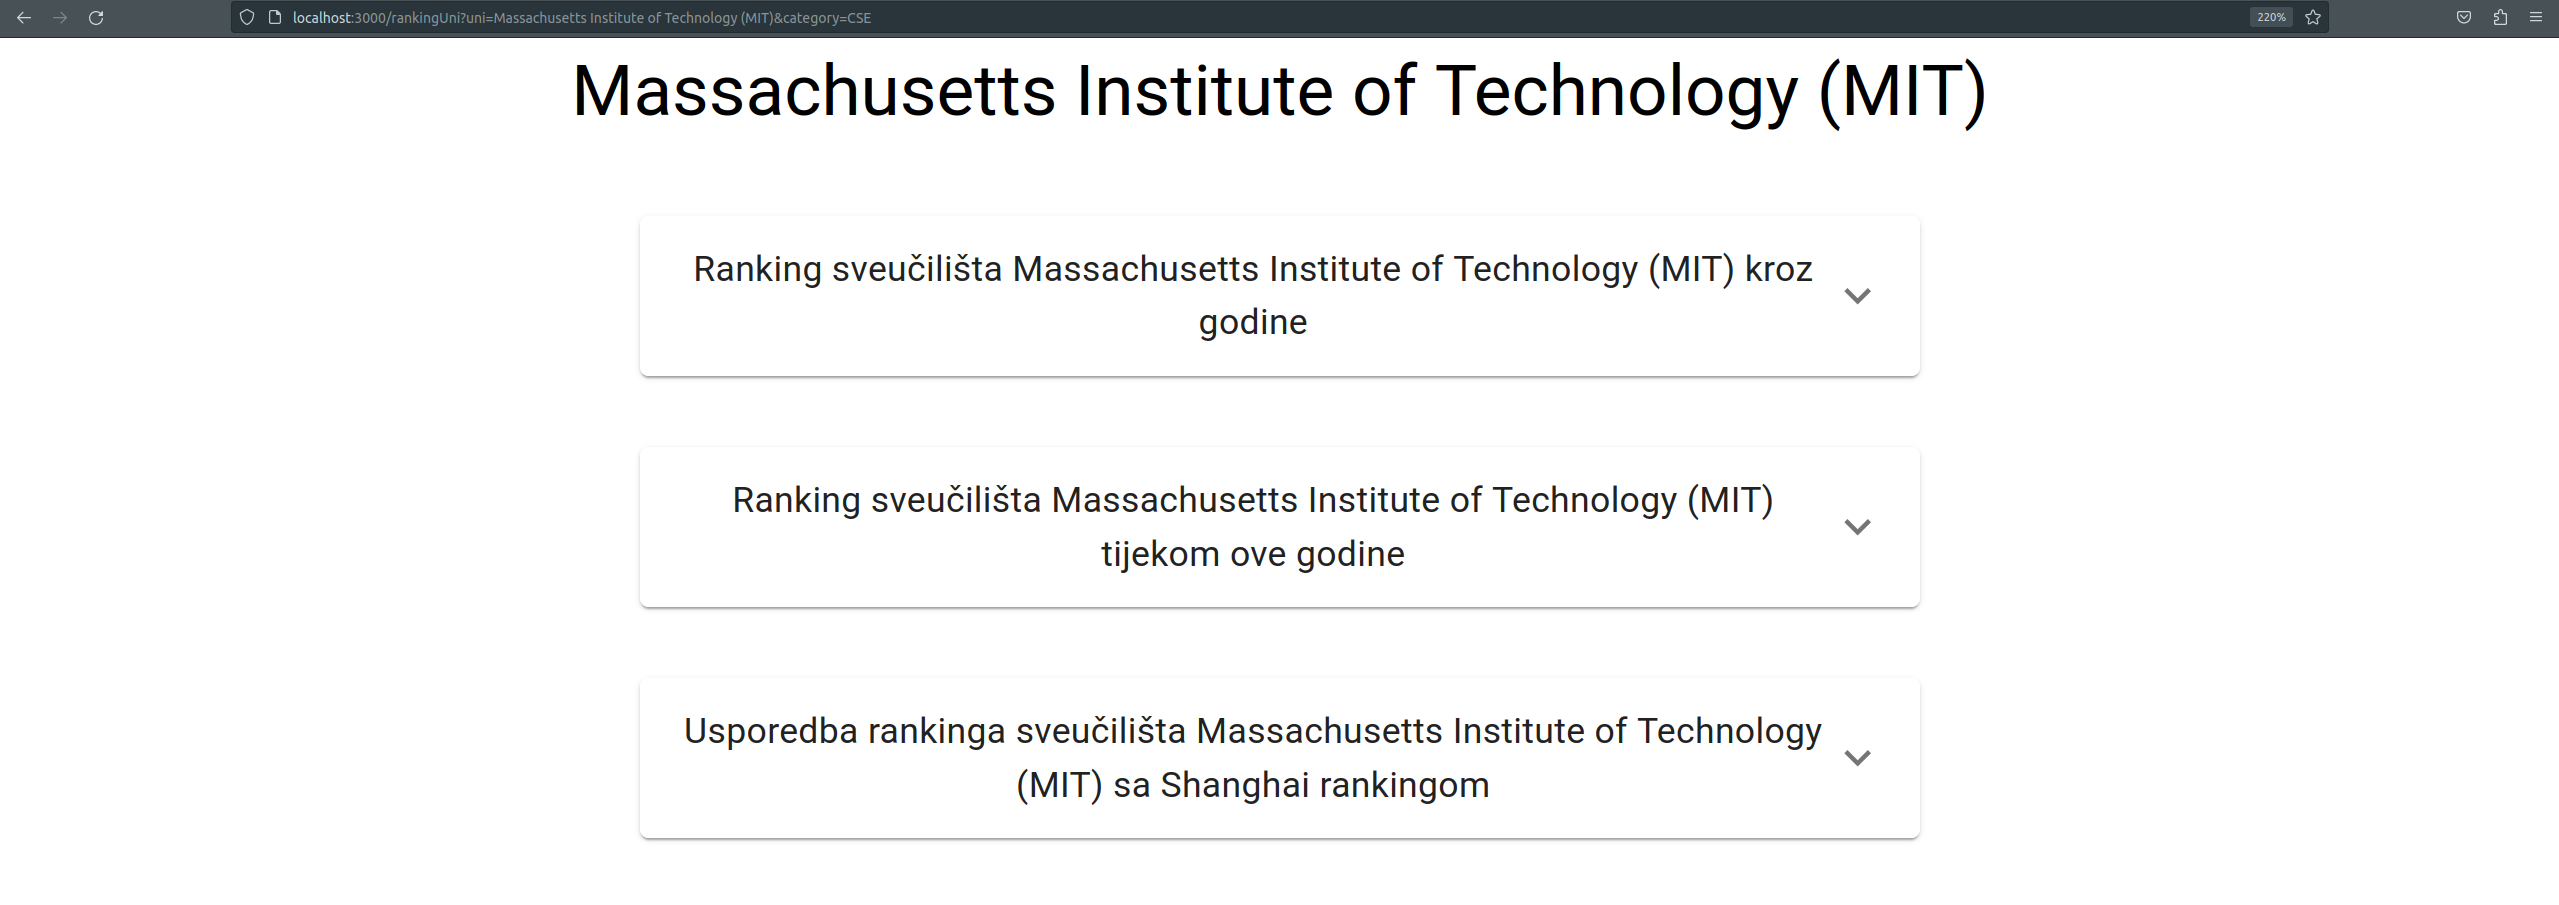
\includegraphics[scale=0.21]{unipage.png} 
       \caption{Stranica sveučilišta}
       \label{fig:unipage}
       \end{figure}
\\Nakon što je korisnik pritisnuo ime nekog sveučilišta prikazat će mu se stranica na slici \ref{fig:unipage}. Stranica sa slike nalazi se na putanji 
"/rankingUni?uni=Massachusetts Institute of Technology (MIT)\&category=CSE". Parametar \emph{uni} specifira za koje sveučilište će se prikazivati podatci, a 
parametar \emph{category} specifira za koje područje se prikazuju podatci. U primjeru sa slike \ref{fig:unipage} gledamo stranicu koja se odnosi na sveučilište 
Massachusetts Institute of Technology (MIT) za područje CSE. Područje za koje promatramo podatke ovisi za koje područje je korisnik prethodno gledao 
rang listu te se ono prenosi na ovu stranicu. 
\\Na ovoj stranici korisnik može birati između 3 ponuđene opcije. 
Pritiskom na prvi padajući izbornik prikazat će se grafički prikaz promjene podataka za ranking 
od 2017. godine, što se vidi na slici \ref{fig:unipage1}. 
\begin{figure}[htb]
    \hspace*{-2cm}  
       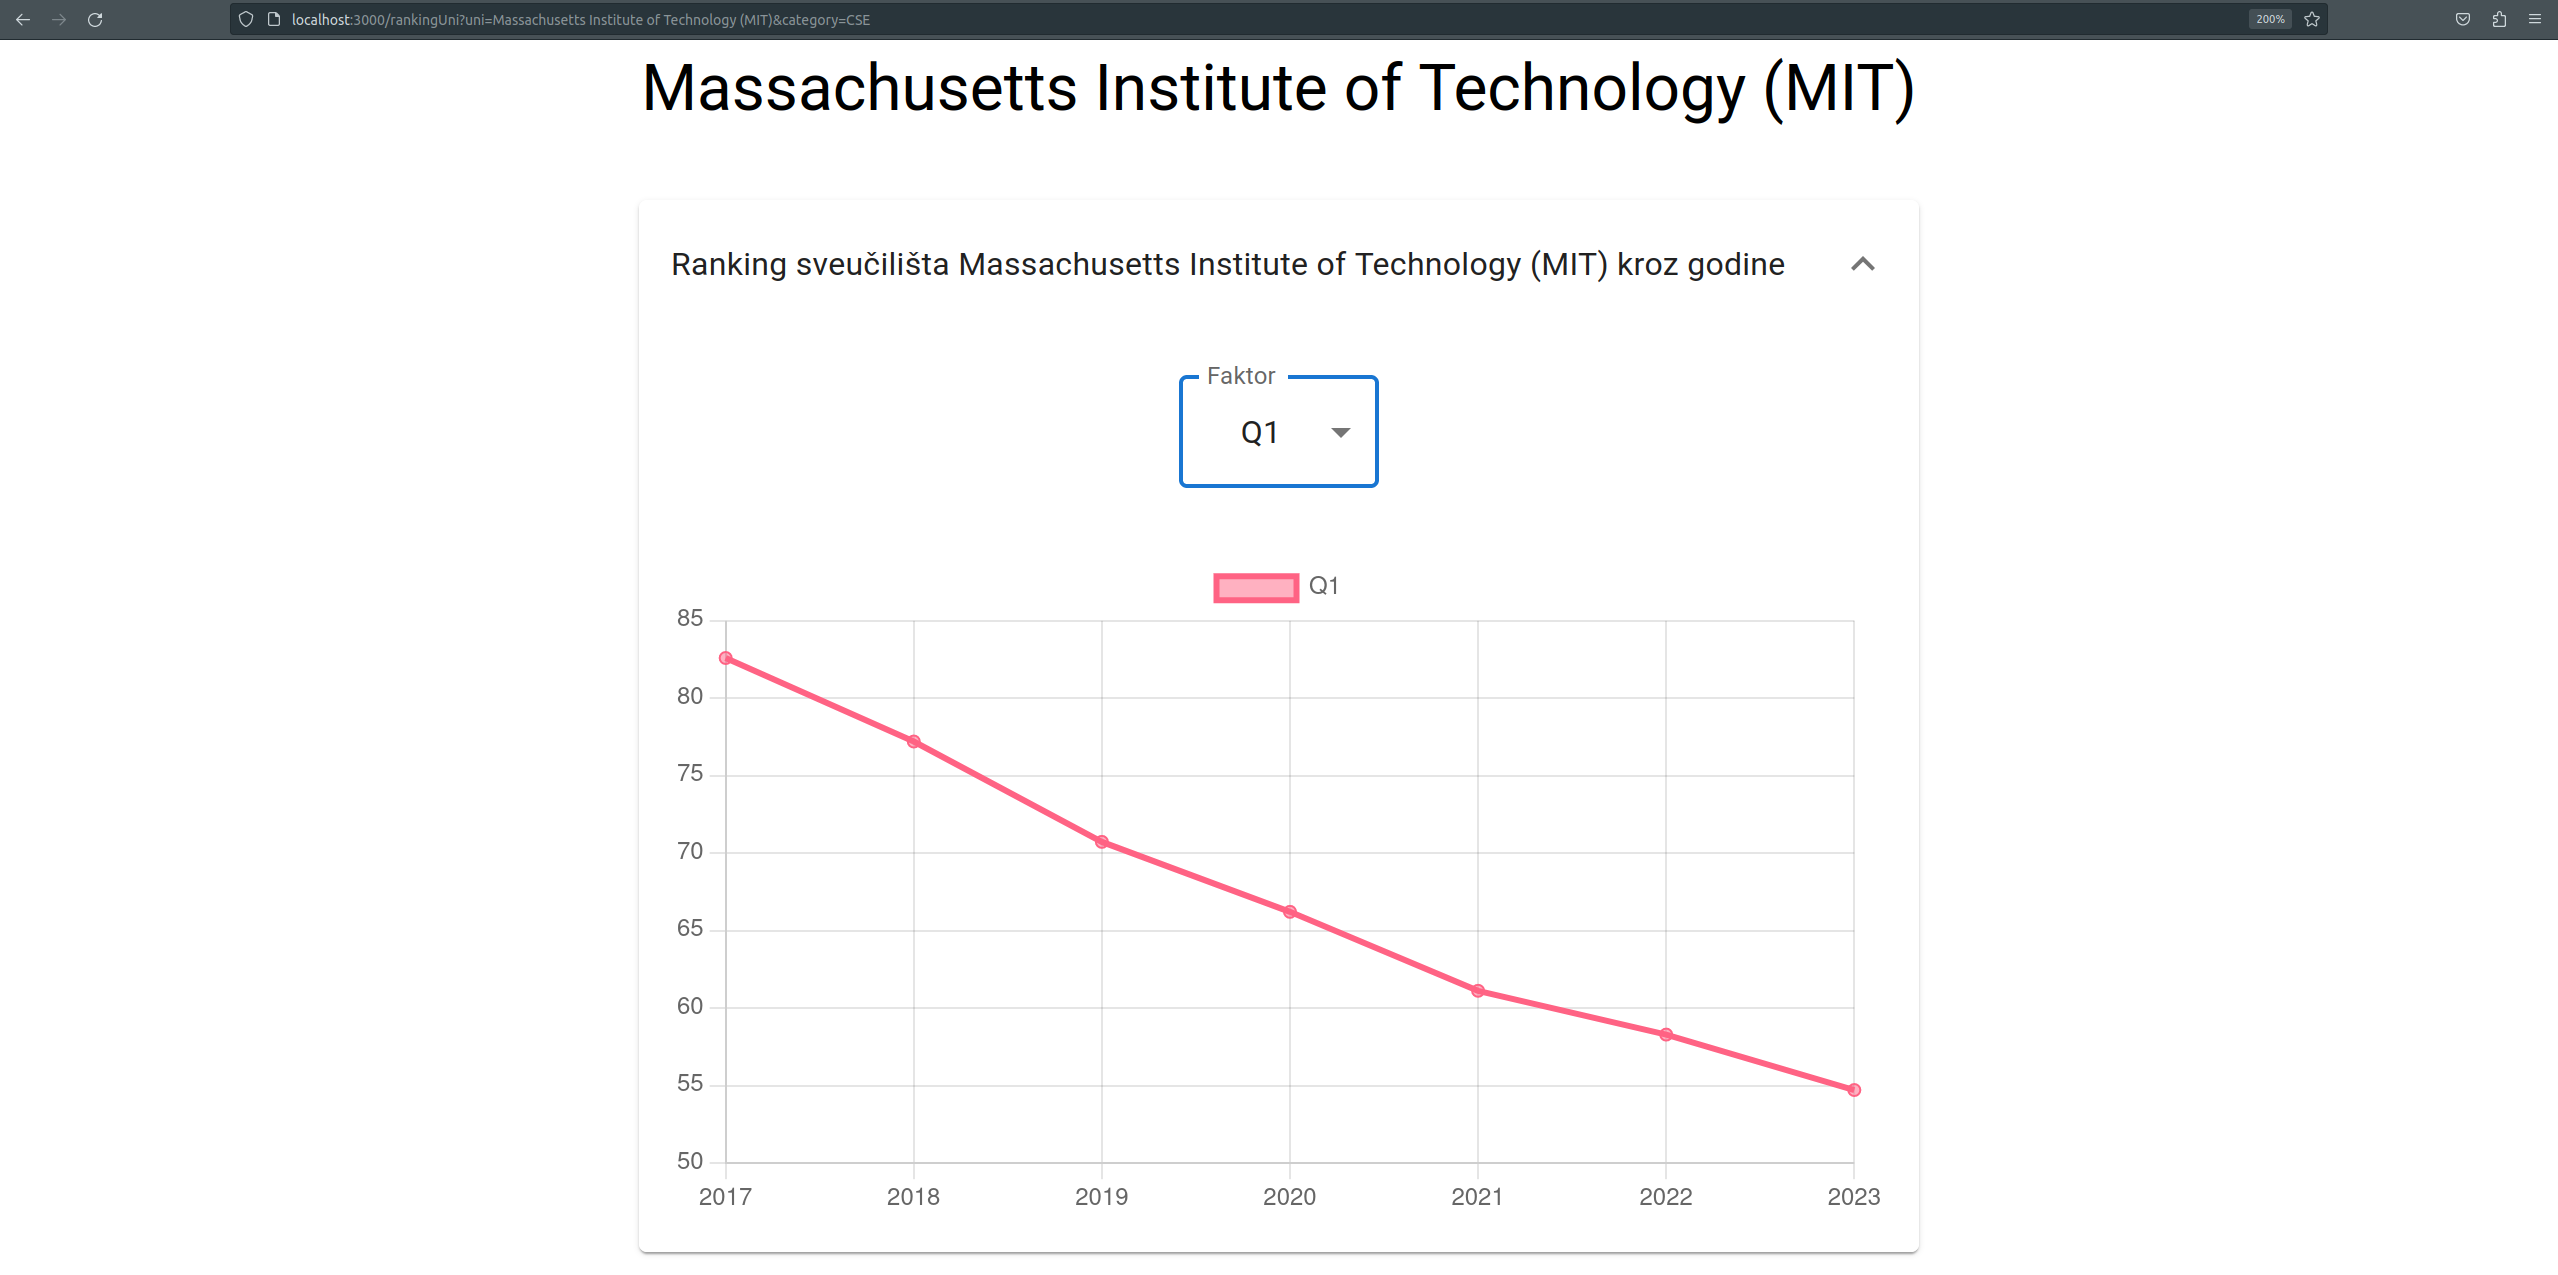
\includegraphics[scale=0.21]{uni1.png} 
       \caption{Grafički prikaz promjene vrijednosti indikatora}
       \label{fig:unipage1}
       \end{figure}
Ukoliko korisnika zanima vrijednost nekog drugog podatka za ranking, na raspolaganju mu je izbornik 
koji je prikazan na slici \ref{fig:unipage2}. 
\begin{figure}[htb]
    \hspace*{-2cm}  
       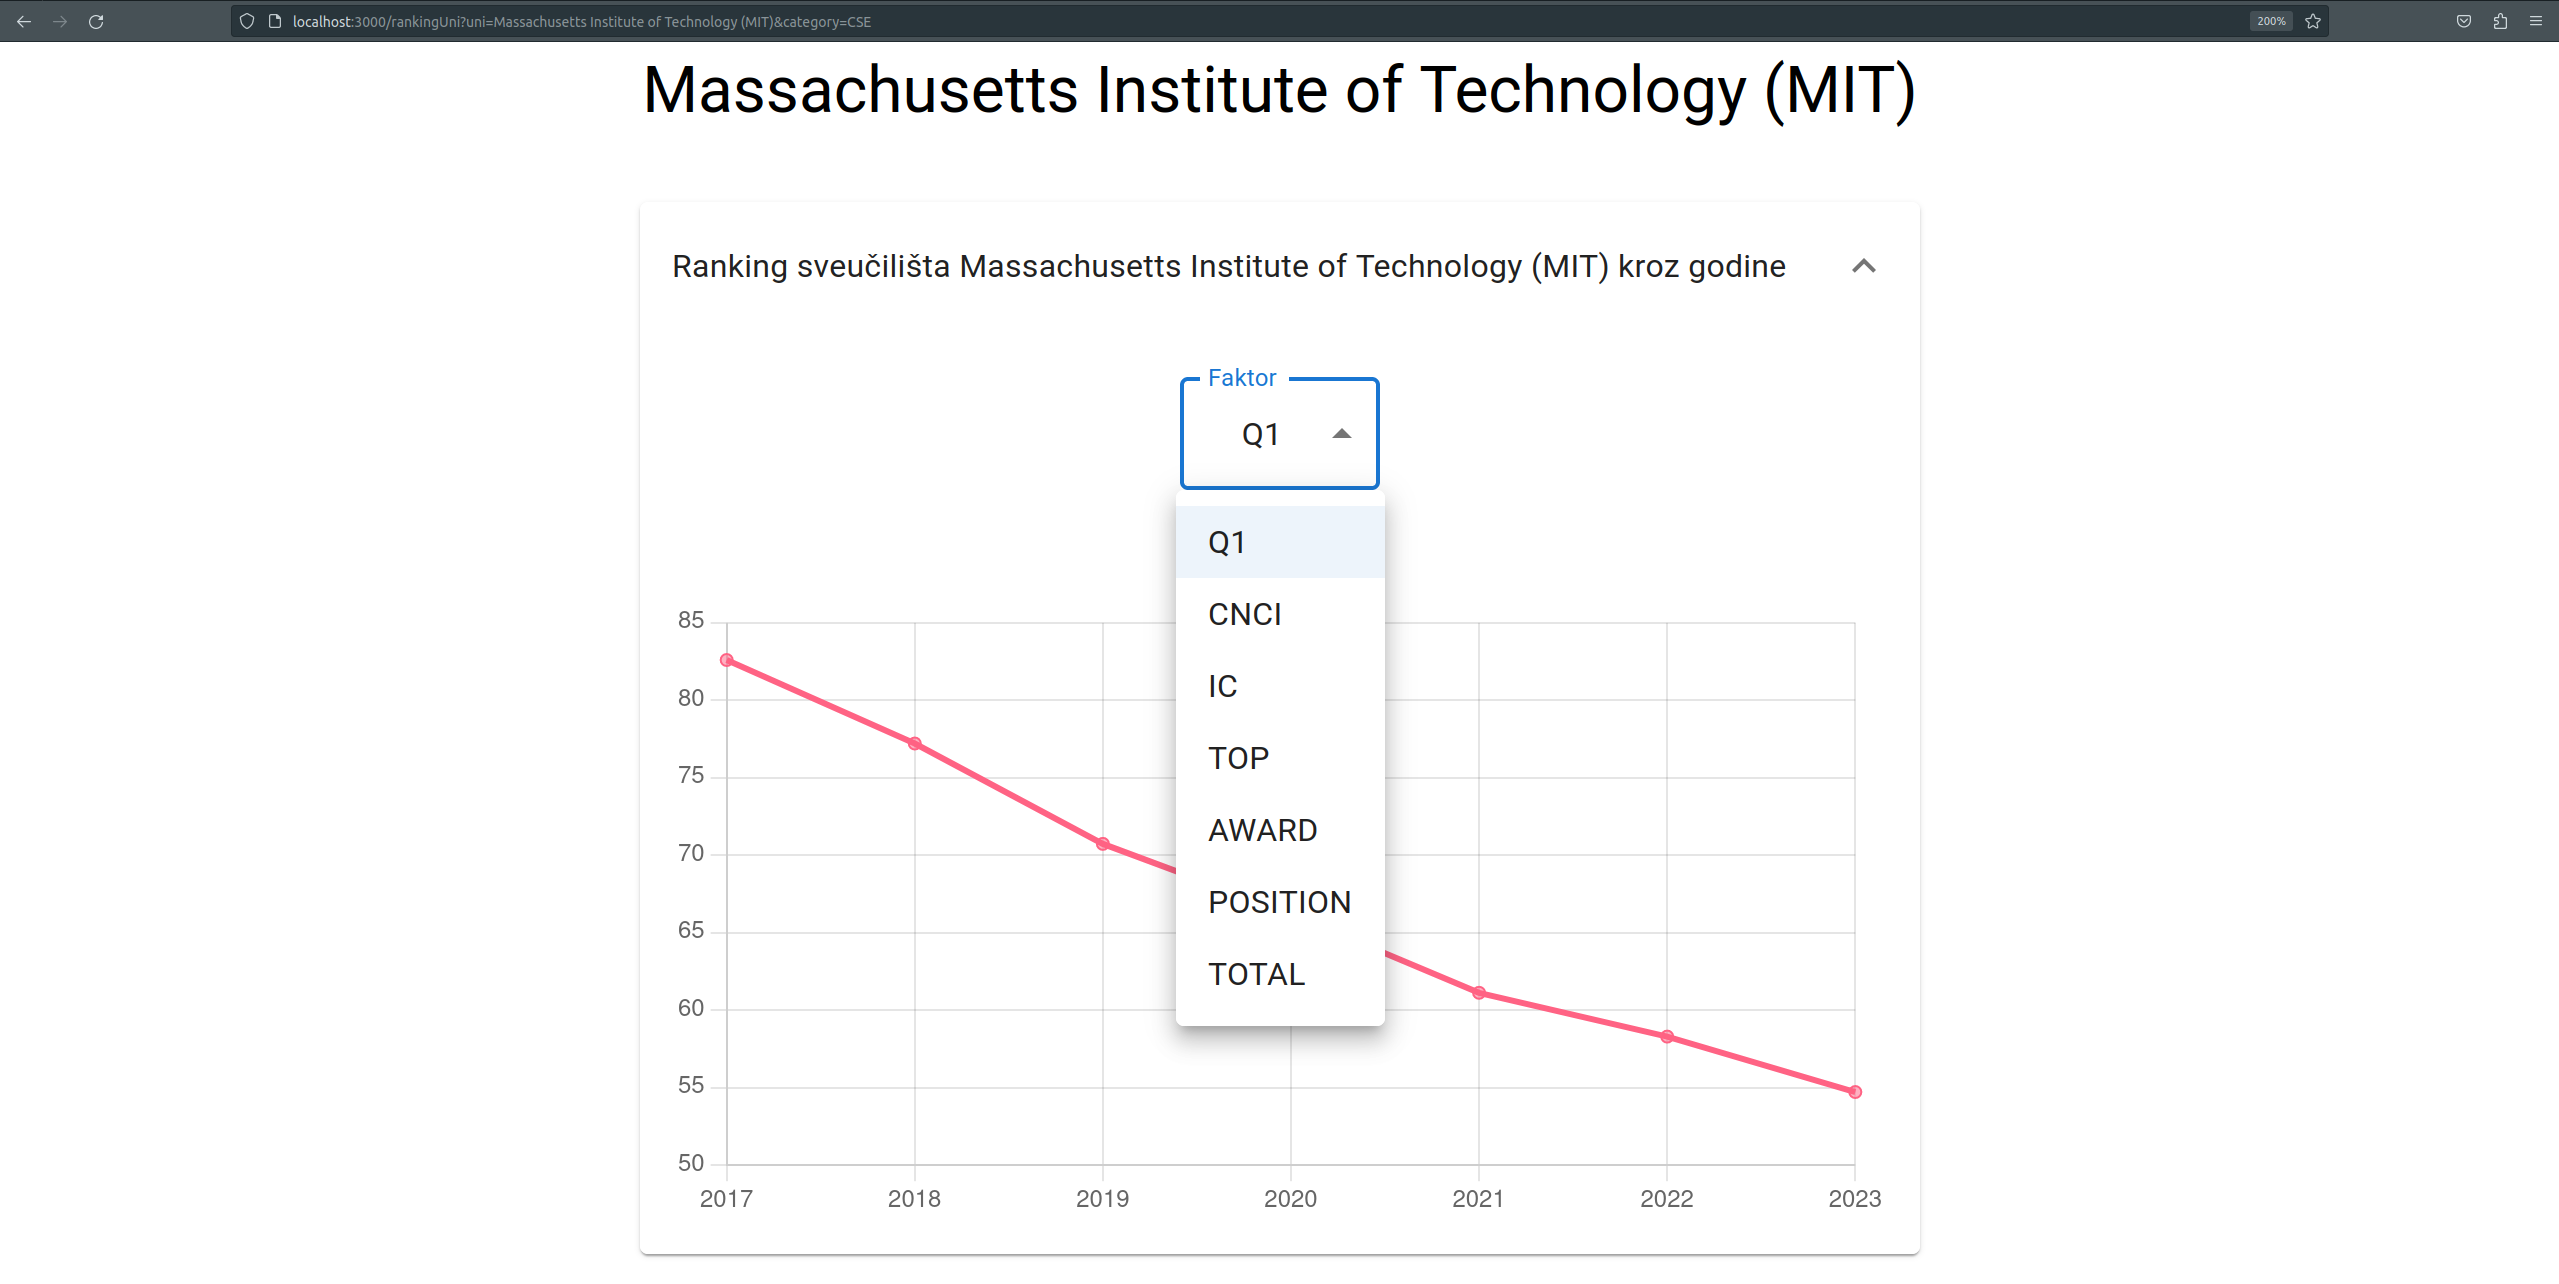
\includegraphics[scale=0.21]{uni2.png} 
       \caption{Grafički prikaz promjene vrijednosti indikatora}
       \label{fig:unipage2}
       \end{figure}
Postoji mogućnost pregleda promjene vrijednosti svih indikatora koji služe za računanje rankinga: Q1, CNCI, IC, Top, Award. 
Osim vrijednosti indikatora može se promatrati kako se pozicija \engl{position} sveučilišta te ukupna vrijednost \engl{total} prema kojoj se sveučilišta 
sortiraju na rang listi mijenjala kroz godine. Iz grafičkog prikaza se ne mogu potpuno točno pročitati vrijednosti podataka za neku godinu. Točan iznos 
nekog podatka za određenu godinu dobije se zadržavanjem miša na krivulji iznad određene godine, što se vidi na slici \ref{fig:detail}.
\begin{figure}[htb]
            \centering
               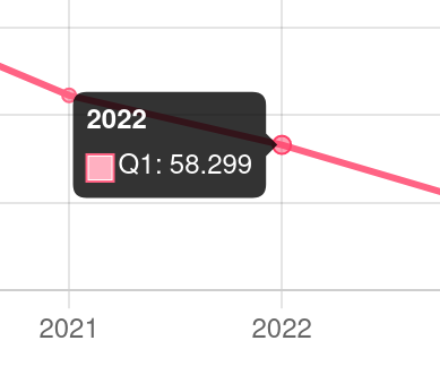
\includegraphics[scale=0.4]{detail.png} 
               \caption{Detaljniji prikaz vrijednosti podataka na grafu}
               \label{fig:detail}
               \end{figure}           
\FloatBarrier 
Pritiskom na drugi padajući izbornik korisniku se prikaže isti graf s opcijom pregleda podataka za ranking
kao i u prethodnom slučaju. Jedina razlika je što ovaj graf prikazan na slici \ref{fig:uni3}
prikazuje promjenu procjene ranking podataka tijekom mjeseci tekuće godine. Primjer sa slike \ref{fig:uni3} nije reprezentativan jer su podatci 
prikupljani u kratkom vremenskom razdoblju, no kada bi se aplikacija držala pokrenutom tijekom jedne godine vidjeli bismo promjene na grafu. Pregledom ovog 
grafa može se procjeniti kako će izgledati Shanghai Ranking rang lista za trenutnu godinu prije službene objave. 
\begin{figure}[htb]
    \hspace*{-2cm}  
       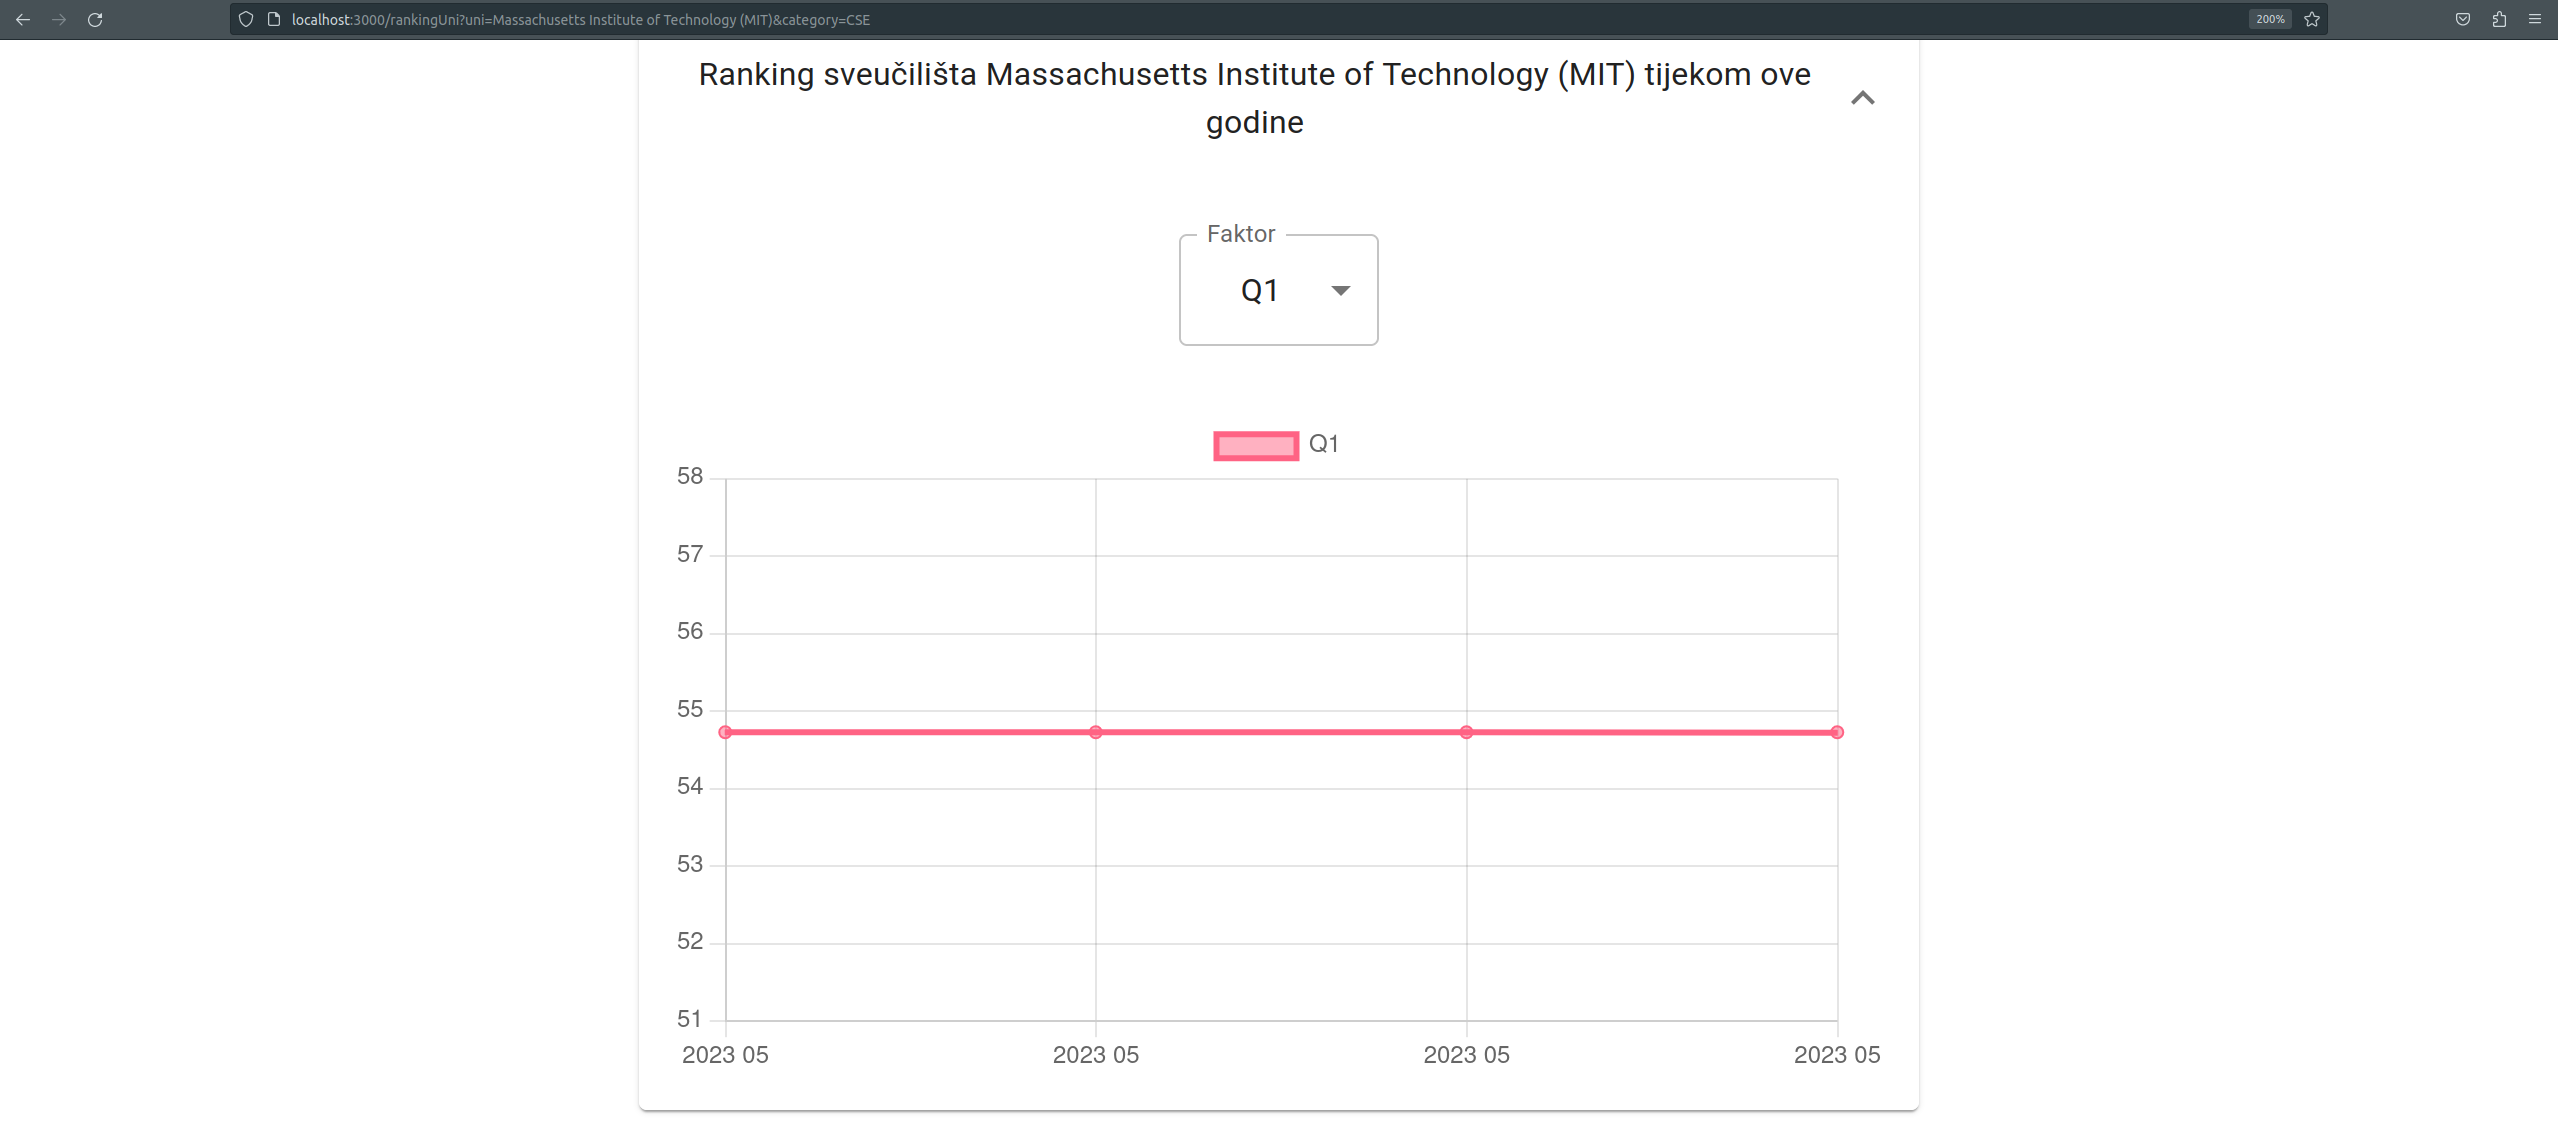
\includegraphics[scale=0.21]{uni3.png} 
       \caption{Prikaz ranking podataka za trenutnu godinu}
       \label{fig:uni3}
       \end{figure} 
\\Pritiskom na treći padajući izbornik prikaže se grafički prikaz na kojem 
\begin{figure}[htb]
    \hspace*{-2cm}  
       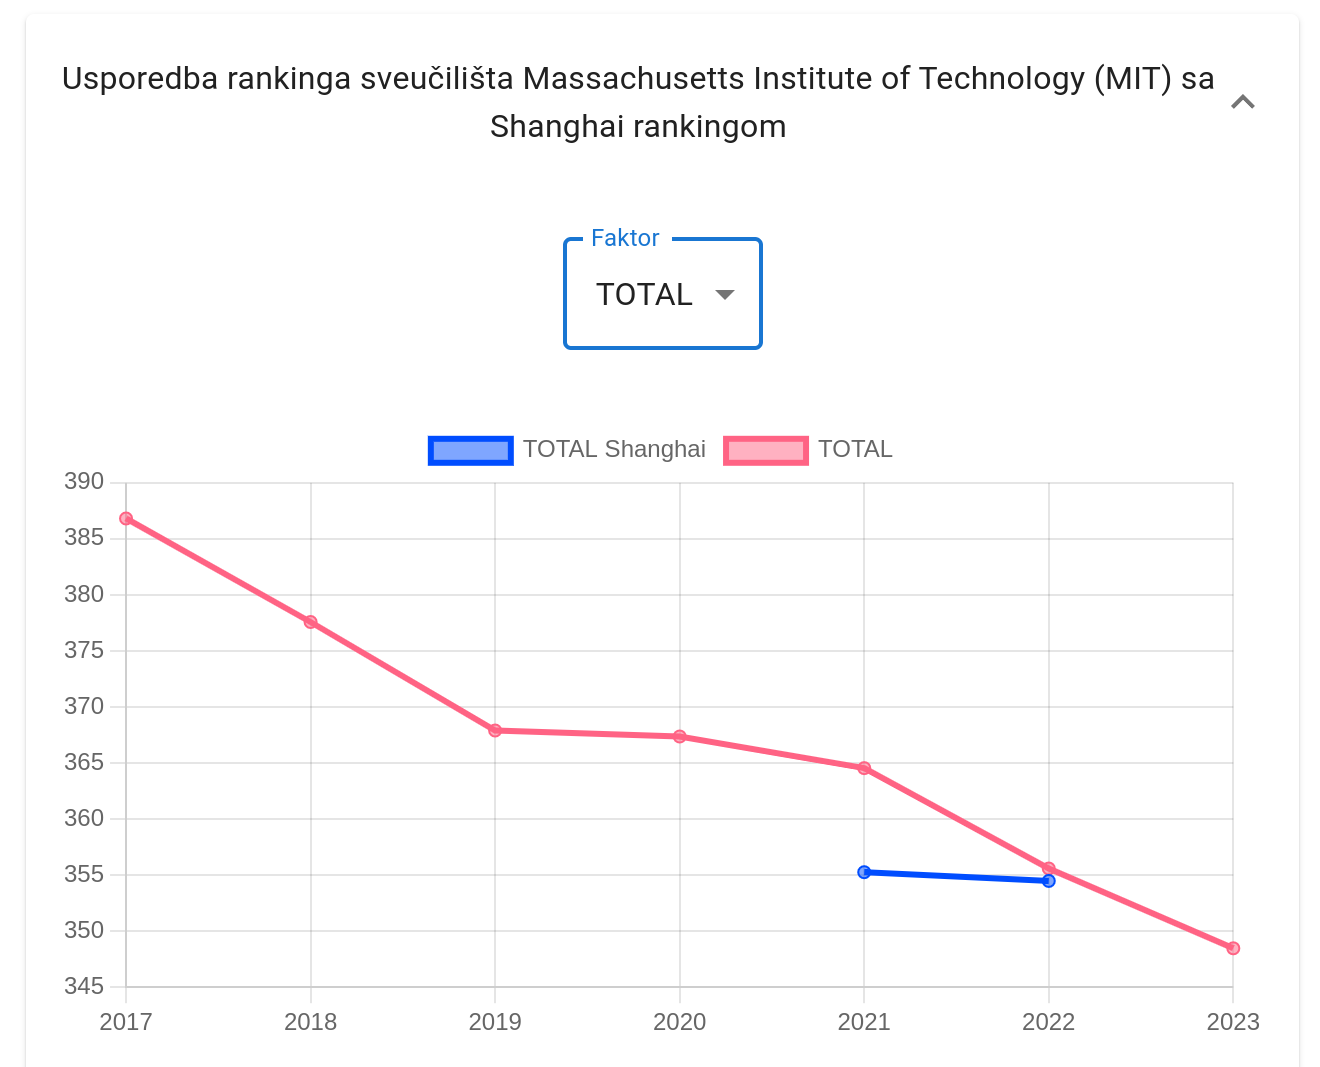
\includegraphics[scale=0.35]{uni4.png} 
       \caption{Grafički prikaz usporedbe procjene rankinga i stvarnih Shanghai Ranking podataka}
       \label{fig:uni4}
       \end{figure} 

\chapter{Zaključak}
Zaključak.

\bibliography{literatura}
\bibliographystyle{fer}

\begin{sazetak}
Sažetak na hrvatskom jeziku.

\kljucnerijeci{Ključne riječi, odvojene zarezima.}
\end{sazetak}

% TODO: Navedite naslov na engleskom jeziku.
\engtitle{Title}
\begin{abstract}
Abstract.

\keywords{Keywords.}
\end{abstract}

\end{document}
